\documentclass[ngerman]{tudscrreprt}
\usepackage{selinput}
\SelectInputMappings{adieresis={ä},germandbls={ß}}
\usepackage[T1]{fontenc}
\usepackage{babel} 
\usepackage{isodate}
\usepackage{amssymb}
\usepackage{amsmath}
\usepackage{float} % lädt das Paket zur Verwendung von zusätzlichen Positionsbefehlen
\usepackage{wrapfig}  
\usepackage{picinpar}   
\usepackage{hyperref}
\usepackage{enumerate}

\begin{document}
\faculty{Fakultät Elektrotechnik und Informationstechnik} \department{} \institute{Institut für Regelungs - und Steuerungstheorie} \chair{Prof. Dr.-Ing. habil. Dipl. Math. Klaus Röbenack} \title{Nichtlineare Regelungstechnik 2{\footnote{Mitschrift von Bolor Khuu}}
}
% \thesis{diss}
% \degree[Dr.-Ing.]{Doktor-Ingenieur}
\author{Prof. Dr.-Ing. habil. Dipl. Math. Klaus Röbenack}
% \dateofbirth{2.1.1990}
% \placeofbirth{Dresden}
\date{\today}
% \defensedate{20.10.2014}
% \referee{Dagobert Duck \and Mac Moneysac}
\maketitle
\tableofcontents
\newpage
\chapter{Einführung}
Nichtlineare Zustandsraummodelle (Systeme gewohnliche Differentialgleichung 1. Ordnung)\\
\begin{figure}[H]
\centering
\def\svgwidth{200pt} 
  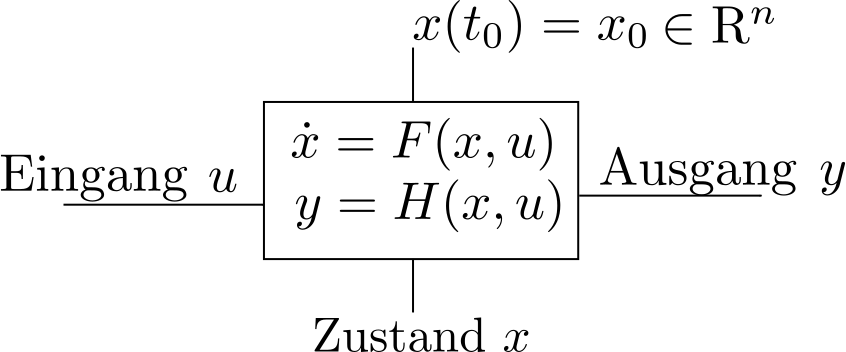
\includegraphics[width=7.5cm]{image1.pdf}
\end{figure}
\begin{equation*}
\begin{matrix}
F:\mathrm{R}^n \times \mathrm{R}^m \to \mathrm{R}^n \\ 
F:\mathrm{R}^n \times \mathrm{R}^m \to \mathrm{R}^p
\end{matrix}
\end{equation*}
Beispiel für diese Systemklasse 
\begin{itemize}
\item Starrkörpermodell
\item Elektrische Netzwerke
\item Chemische Reaktoren mit idealer Durchmischung
\end{itemize}
\section{Systembeschreibung, Einführungsbeispiele}
\subsection*{\textbf{Beispiel}. 1.1: Kinematisches Modell eines mobilen Roboters}
\begin{figure}[H]
\centering
\def\svgwidth{200pt} 
  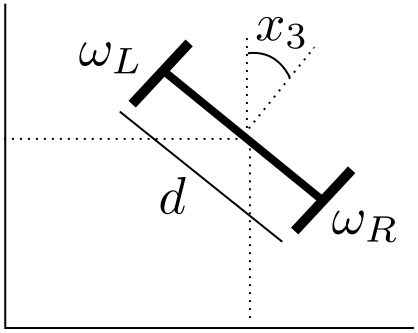
\includegraphics[width=5.5cm]{image2.pdf}
\end{figure}
Antrieb: $\omega_L, \omega_R \dots$ Winkelgeschwindigkeit links, rechts Rad
\begin{equation*}
\begin{matrix}
u_1 &=& \frac{r}{2}(\omega_L + \omega_R) &\to &\text{translatorischer Anteil}\\ 
u_2 &=& \frac{r}{d}(\omega_L - \omega_R) &\to &\text{rotatorischer Anteil}
\end{matrix}
\end{equation*}
$r\dots$  Radius der Räder\\ 
$d\dots$  Achsenlänge\\ 

\begin{equation*}
\begin{pmatrix}
\dot{x}_1 \\ 
\dot{x}_2\\ 
\dot x_3
\end{pmatrix}=
\underbrace{
\begin{pmatrix}
\sin{x_3} \\ 
\cos{x_3}\\ 
0
\end{pmatrix}}_{\text{transl.Bew}}\cdot u_1 + 
\underbrace{
\begin{pmatrix}
0\\ 0\\ 1
\end{pmatrix}}_{\text{rot.Bew}} \cdot u_2
\end{equation*}
Ausgang: Position in der Ebene
\begin{equation*}
\begin{matrix}
y_1 = x_1\\
y_2 = x_2
\end{matrix}
\end{equation*}
\subsection*{\textbf{Beispiel}. 1.2: Hochsteller (Boost Converter)}
Spannung in Masche
\begin{equation*}
L\dot I = E + \left\{ 
\begin{matrix}
0 , \quad d=1\\ 
-u, \quad d=0
\end{matrix}
\right .
\end{equation*}
Ströme im Knoten 
\begin{equation*}
C\dot U = -\frac{U}{R} + \left\{ 
\begin{matrix}
I, \quad d=0\\ 
0, \quad d=1
\end{matrix}
\right .
\end{equation*}
Zustand 
\begin{equation*}
x = \begin{pmatrix} x_1\\ x_2 \end{pmatrix} = (\frac{I}{U})
\end{equation*}


\begin{equation*}
\begin{matrix}
\dot x_1 &=& -(1-d) \frac{1}{L}x_2 + \frac{E}{L}\\ 
\dot x_2 &=& (1-d) \frac{1}{C} x_1 - \frac{1}{RC}x_2
\end{matrix}
\end{equation*}
Signalbereich für $d$:\\  
$d\in [ 0, 1]$: Ideales Schalten $\Rightarrow$ linear, aber ereignisdiskret\\ 
$d\in [ 0,1 ]$: Mitteilung, PWM $\Rightarrow$ zeitkontinieurlich, aber nichtlinear
\chapter{Grundlagen}
\section{Lineare Algebra}
\begin{itemize}
\item $n-$dim , reeller Vektorraum\footnote{VR = Vektorraum} $\mathrm{R}^n$ Elemente: Vektoren bzw. Spaltenvektoren
\begin{equation*}
x\in \mathrm{R}^n , \qquad x = \begin{pmatrix} x_1 \\ \vdots\\ x_n \end{pmatrix} 
\end{equation*} 
\item Einheitsvektoren 
\begin{equation*}
e_1 = 
\begin{pmatrix}
1\\ 0\\ \vdots\\ 0
\end{pmatrix} , \dots, 
e_n=
\begin{pmatrix}
0\\ \vdots\\ 0\\ 1
\end{pmatrix}
\end{equation*}
bilden Basis des $\mathrm{R}^n$ Standartbasis
\item Jeder Vektor $x\in \mathrm{R}^n$ läßt sich eindeutig als Linearkombination der Basisvektoren darstellen
\begin{equation*}
x = x_1 e_1 + \dots + x_n e_n
\end{equation*}
\item Lineare Hütte von $r$ Vektoren $v_1 , \dots, v_r \in \mathrm{R}^n$ ist die Menge aller Linearkombination: 
\begin{equation*}
\text{span}\{ v_1, \dots, v_r \} = \{ \alpha_1 v_1 + \dots \alpha_r v_r | \alpha_1, \dots, \alpha_r \in \mathrm{R} \}
\end{equation*}
Die lineare Hütte ist ein Untervektorraum \footnote{UVR = Untervektorraum} des $\mathrm{R}^n$
\item $m\times n$ -Matrix $A \in \mathrm{R}^{m\times n}$
\begin{equation*}
A= 
\begin{pmatrix}
a_{11} &\dots &a_{1n}\\ 
\vdots &\ddots &\vdots\\ 
a_{m1} &\dots &a_{mn}
\end{pmatrix}
\end{equation*}
\item Bild(image,range) einer Matrix $A$:
\begin{equation*}
\begin{matrix}
\text{im}A &=& \{y\in \mathrm{R}^m : \exists \times \in \mathrm{R}^n \quad \text{mit}\quad y= Ax \} \\ 
&=& \{ (Ax)\in \mathrm{R}^m |\forall \times \in \mathrm{R}^n \}
\end{matrix}
\end{equation*}
A spaltenweise
\begin{align*}
A =& (v_1 ,\dots, v_n )\in \mathrm{R}^{m\times n}\\
 &(v_1 ,\dots, v_m )\in \mathrm{R}^{m\times m}
\end{align*}
Linearkombination: 
\begin{equation*}
Ax= x_1 v_1 + \dots + x_n v_n 
\end{equation*}
Es gilt: $\text{im} = \text{span}\{ v_1, \dots , v_n \}$ 

\item Kern (kernel, null space) der Matrix $A$:
\begin{equation*}
\text{ker}A = \{ x\in \mathrm{R}^n | Ax = 0 \}
\end{equation*}
\item $\text{im}A$ ist UVR des $\mathrm{R}^m$, \\ 
Rang: $\text{rang} A = \text{dim}(\text{im}A)$
\item $\text{ker}A$ ist UVR des $\mathrm{R}^n$
\item Zerlegungen: 
\begin{equation*}
\begin{matrix}
\mathrm{R}^m &=& \text{im}A &\overset{\text{direkte Summe}}{\oplus} &\text{ker} A^T \\ 
\mathrm{R}^n &=& \text{ker}A& \oplus &\text{ker} A^T 
\end{matrix}
\end{equation*}


\item Die Matrix $A \in \mathrm{R}^{m\times n}$ wird mit unter synonym in lin. Abb. (lineare Operator) behandelt:
\begin{equation*}
\begin{matrix}
\textit{A}&: &x \to A x\\ 
\textit{A}&: &\mathrm{R}^n \to \mathrm{R}^m
\end{matrix}
\end{equation*}
Notation: $\textit{A}\in L (\mathrm{R}^n, \mathrm{R}^m)$
\item Der Dualraum $(\mathrm{R}^n)^*$ des $\mathrm{R}^n$ besteht aus dem auf $\mathrm{R}^n$ definierten linearen Funktionalen\\ (Linearformen):$(\mathrm{R}^n)^* = L(\mathrm{R}^n, \mathrm{R})$
\begin{equation*}
\underbrace{(\omega_1, \dots, \omega_n)}_{\omega\in \mathrm{R}^{n*}} \cdot 
\underbrace{\begin{pmatrix}
x_1 \\ \vdots\\ x_n
\end{pmatrix}
}_{x\in \mathrm{R}^n} = y \in \mathrm{R}
\end{equation*}
Darstellung durch Zeilenvektoren der Form $\omega = (\omega_1, \dots, \omega_n)$, die man auch Kovektoren nimmt.
\item der Dualraum ist selber ein n-dim. reeller VR. Standartbasis (Kanonische Basis)
\begin{equation*}
\begin{matrix}
e_1^* &=& (1, 0, \dots, 0)\\ 
e_1^* &=&(0, \dots, 0, 1)
\end{matrix}
\end{equation*}
Darstellung von $\omega$. \begin{equation*}
\omega= \omega_1 e_1^* + \dots + \omega_n e_n^*
\end{equation*}
\item Inneres Produkt (Skalarprodukt)
\begin{equation*}
\langle \cdot, \cdot \rangle : (\mathrm{R}^n)^* \times \mathrm{R}^n \to \mathrm{R}
\end{equation*}
mit 
\begin{equation*}
\begin{matrix}
\langle \omega, x\rangle &=&\omega x\\ 
&=&(\omega_1, \dots, \omega_n)\begin{pmatrix} x_1\\ \vdots\\ x_n \end{pmatrix}\\ 
&=& \sum\limits_{i=1}^n \omega_i x_i

\end{matrix}
\end{equation*}
\begin{equation*}
\begin{matrix}
\langle \omega, e_j \rangle = \omega_j \\ 
\langle e_i^*, x\rangle = x_i
\end{matrix}
\end{equation*}
\item Die Basis $\{e_1^*, \dots, e_n^*\}$ ist die zu $\{ e_1, \dots, e_n \}$ duale Basis, d.h. 
\begin{equation*}
\langle e_i^*, e_j \rangle = \delta_{ij} \qquad ; 1\le i, j\ge n
\end{equation*}
mit dem Kroneckersymbol 
\begin{equation*}
\left\{ 
  \begin{array}{l l}
    1 & \quad \text{ für } i = j\\
    0 & \quad \text{ sonst }
  \end{array} \right.
\end{equation*}
\end{itemize}
\section{Felder und Ableitungen}
Sei $M \in \mathrm{R}^n$ offen. \\ 
\begin{equation*}
\begin{array}{ll}
h: M \to \mathrm{R} &\dots \text{Skalarfeld}\\ 
f: M \to \mathrm{R}^n &\dots \text{Vektorfeld}\\ 
\omega: M \to (\mathrm{R}^n)^* &\dots \text{Kovektorfeld}\\ 
&\dots \text{Differentialform}\\ 
& \quad (\sim \text{1. Grades})\\ 
&\quad(\text{1. Form, Pfaffsche Form})
\end{array}
\end{equation*}
\begin{itemize}
\item Neben Darstellung eines Vektorfeldes als Spaltenvektor 

\begin{equation*}
f(x) = \begin{pmatrix}
f_1(x)\\ \vdots\\ f_n(x)
\end{pmatrix}
\end{equation*} wird auch die Notation 
\begin{equation*}
f(x) = f_1(x) \frac{\partial}{\partial x_1} + \dots + f_n(x)\frac{\partial}{\partial x_n}
\end{equation*}
verwendet. \begin{equation*}
\left\{
\frac{\partial }{\partial x_1}, \dots , \frac{\partial }{\partial x_n}
\right\} \text{Kanonische Basis}
\end{equation*} 
\begin{figure}[H]
\centering
\def\svgwidth{200pt} 
  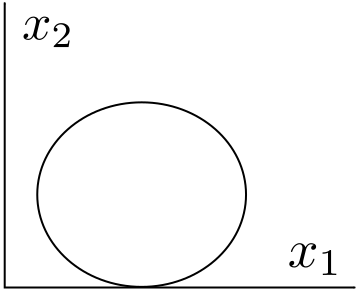
\includegraphics[width=3.5cm]{image17_1.pdf}
\end{figure}
Zugehörige duale Basis: \begin{equation*}
\left\{ 
dx_1,\dots, dx_n
\right\}
\end{equation*}
Kovektorfeld $\omega:$ Zeilenvektor \begin{equation*}
\omega (x) = (\omega_1 (x) , \dots,\omega_n(x) )
\end{equation*} 
oder 
\begin{equation*}
\omega (x) = (\omega_1 (x) dx_1 + \dots + \omega_n(x)dx_n )
\end{equation*} 
\item Jacobimatrix, vektorielle Funktion
\begin{equation*}
\begin{array}{l l }
F: M \to \mathrm{R}^m & \\ 
F'(x) = dF(x) & = 
\begin{pmatrix}
\frac{\partial F_1}{\partial x_1}(x) &\dots& \frac{\partial F_1}{\partial x_n}(x)\\ 
\vdots & \ddots & \vdots \\ 
\frac{\partial F_m}{\partial x_1}(x)&\dots & \frac{\partial F_m}{\partial x_n}(x)
\end{pmatrix} \in \mathrm{R}^{m\times n}
\end{array}
\end{equation*} 
\item Gradient bzw. Differential eines Skalarfelds $h$ 
\begin{equation*}
h'(x) = dh(x) = \left( \frac{dh}{dx_1}, \dots, \frac{dh}{dx_n} \right) \in (\mathrm{R}^n)^*
\end{equation*}
Gradient ist ein Kovektorfeld (KVF)
läßt sich ein KVF als Gradient eines Skalarfelds (SF) darstellen, so heißt es exakte Differential, exakte 1-Form, $\dots$ Das zugehörige SF heißt Potential.
\item Hessematrix des Skalarfelds $h$: 
\begin{equation*}
h^{''}(x) = \begin{pmatrix}
\frac{\partial^2 h}{\partial x_1^2} & \dots & \frac{\partial^2h}{\partial x_1\partial x_n}\\ 
\vdots& \ddots \vdots \\
\frac{\partial^2 h}{\partial x_n^2} & \dots & \frac{\partial^2h}{\partial x_n\partial x_n^2}
\end{pmatrix} \in \mathrm{R}^{n\times m}
\end{equation*}
\end{itemize}
\subsection*{Lemma/Satz von Schwarz:} 
Das SF 
$h: M\to \mathrm{R}$ sei im Pkt $p\in M$ zweimal stetig diffbar, Dann gilt: \begin{equation*}
\frac{\partial^2h}{dx_i \partial x_j}(p) = \frac{\partial^2h}{\partial x_j \partial x_i} \text{  für  } i,j = i,j=1,\dots, n.
\end{equation*}
\subsection*{Pioncaresches Lemma:} Sei $\omega: M \to (\mathrm{R}^n)^* $ ein stetig diffbares KVF und 
\begin{equation*}
U = B_r (p) = \{ x\in M | \quad \|{x-p}< r\|\quad \} , r>0.
\end{equation*}
Diffentialform $\omega$ ist auf $U$ genau dann exakt, wenn 

\begin{equation*}
\frac{\partial \omega_i}{\partial x_j}(x) = \frac{\partial \omega_j}{\partial x_i}(x) \qquad \forall x\in U \text{ und all } i,j =1,\dots, n.
\end{equation*}
\textbf{Beispiel}: \begin{equation*}
\begin{split}
\omega (x) &= \underbrace{3x^2y^2}_{\omega_1}dx +\underbrace{2x^3 y}_{\omega_2}dy \\ 
&=(3x^2y^2, \quad 2x^3 y)\\ 
\frac{\partial}{\partial y}3x^2y^2 &=6x^2y \text{  exakt } \\ 
\frac{\partial}{\partial x}2x^3 y&= 6x^2y \text{  exakt}
\end{split}
\end{equation*}
Potential: 
\begin{equation*}
\begin{split}
h(x)&= x^3 y^2 \\ 
dh(x)&=(3x^2y^2, \quad 2x^3 y)
\end{split}
\end{equation*}
Beweis: $\Rightarrow \omega$ sei. d.h. $\exists$ SF $h: U\to \mathrm{R}$ mit $dh = \omega$ bzw. $w_i = \frac{\partial h}{\partial x_i}$ 
Dann gilt. \begin{equation*}
\frac{\partial \omega_i}{\partial x_j} = \frac{\partial^2h}{\partial x_j \partial x_i} = \frac{\partial^2h}{\partial x_i \partial x_j} \underset{\text{Schwartz}}{=} \frac{\partial \omega_j}{\partial x_i}
\end{equation*}
Sei $x\in U$. Die Verbindungsstrecke $\{ (1-t)p + tx | 0\le t\le 1  \}$ liegt ganz in $U$ . O.E. sei $p=0$. Ansatz: 
\begin{equation*}
h(x) = \int_0^1 (\sum_{i=1}^n \omega_i (tx)x_i )dt \qquad \forall x \in U \Rightarrow \frac{\partial h}{\partial x_{k}} = \omega_k
\end{equation*}
\section{Vektorfelder und Flüße}
Sei $M \subseteq \mathrm{R}^n$ offen,\\
$F: M \times \mathrm{R} \to \mathrm{R}^n$ ein zeitabhängige Vektorfeld (VF). Anfangswertsaufgabe (AWA) mit Anfangszeitpunkt $t_0\in \mathrm{R}$ und Anfangswert $p \in M:$ \begin{equation*}
\dot x = F(x,t), \quad x(t_0) = p \quad \text{AWA1}
\end{equation*} 
Sei $\mathrm{I} \subseteq \mathrm{R}$ ein offene Intervall im $t_0$. \\ 
Eine diffbare Funktion. $\phi: . \mathrm{I} \to M$ heißt Lokale Lösung von (AWA1) wenn \begin{equation*}
\begin{split}
\dot \phi(t) &=F(\phi(t),t) \quad \forall t\in \mathrm{I}\\ 
\phi(t_0) &= p.
\end{split}
\end{equation*}
Existenzsätze: \begin{itemize}
\item 1. Reano: Sei $F$ stetig. Dann existiert eine (lokale) Lösung der (AWA1), aber nicht unbedingt eindeutig. 
\item 2. Picard-Lindelöff: $F$ geringe zusätzlich eine Lipschitz-Bed. in 1.Argument,
$\exists L \ge 0: \|F(x,t) - F(y,t)\| \le L\cdot \quad \|x-y\| $, 
dann existiert eine lokale eindeutige Lösung von (AWA1).
\end{itemize}
Beweisidee zu 2: (AWA1) ist gleichwertig mit Integralgleichung 
\begin{equation*}
\underbrace{x_{k+1}}_{\text{Picard-Iteration mit $x_0(t)\equiv p$}} = \underbrace{p}_{=x(t_0)} + \int_{t_0}^{t} F(x_k (\tau),\tau)d\tau
\end{equation*}
Folgerung aus Mittelwertsatz der Differentialrechnung: \\ 
Sei $F: M\times \mathrm{R} \to \mathrm{R}^n$ stetig diffbar. Dann genügt $F$ auf jede kompakten Teilmenge $K \subset M\times \mathrm{R}$ einer Litpschitz-Bed. mit der Lipschitz-Konstanten. 
\begin{equation*}
L: = \text{max}_{(x,t)\in K} \| \frac{\partial f(x,t)}{\partial x} \| < \infty
\end{equation*} 
$\Rightarrow$ Lipschitz Bedingung ist lokal erfüllt.\\
\textbf{Beispiel}: $F(x,t)  = x^2$\\ 
$\Rightarrow \dot x = x^2 , \quad x\underbrace{(0)}_{=t_0} = p > 0$ 
\begin{equation*}
\frac{dx}{dt} \Rightarrow \frac{dy}{y^2}|_p^x = d\tau |_0^t \Rightarrow x(t) = \phi(t) = \frac{p}{1-t_p}
\end{equation*}
Existenzintervall $I = \{ -\infty, \frac{1}{p}\}$
\begin{figure}[H]
\centering
\def\svgwidth{200pt} 
  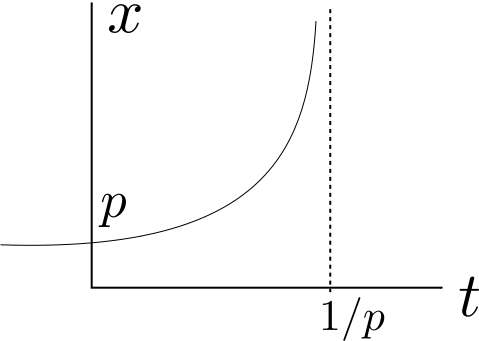
\includegraphics[width=4.5cm]{image17_2.pdf}
\end{figure}
Sei $M \subseteq \mathrm{R}^{n}$ offen, $f,:M \to \mathrm{R}^{n}$ ein Vektorfeld, Dgl \begin{equation*}
\dot x= f(x)
\end{equation*}
\subsection*{Satz(Folgerung von Picard-Lindelöff)}
Das Vektorfeld $f$ sei stetig diffbar.Für jedes $p \in M$ existiert dann ein Intervall $I_p$ um 0, eine offene Kugel $U_p \subseteq M$ um $p$ sowie eine stetig diffbare Abbildung $\varphi: I_p \times U_p \to M$ mit 
\begin{itemize}
\item{1.} Lösung der Dgl:
\begin{equation*}
\frac{\partial}{\partial t}\varphi(t,x) \equiv f(\dot{\varphi}(t,x)) ,\quad \forall t\in I_p \forall x \in U_p
\end{equation*}
\item{2.} Verträglichkeit mit Anfangsbedingungen:
\begin{equation*}
\varphi(0,x) = x, \quad \forall x \in U_p
\end{equation*}
\item{3.} Eindeutigkeit: Jede andere Lösung , die 1. und 2. erfüllt, stimmt für kleine $|t|$ mit $\varphi$ überein.
\end{itemize}
\subsection*{Bemerkung}
\begin{itemize}
\item Die Abbildung $\varphi$ heißt Fluss des VF $f$ (bzw. der Dgl) und ist die allg. Lösung. Notation: $\varphi_t(\cdot) = \varphi(t,\cdot)$
\item Zu jedem Anfangswert $p$ ex. ein maximales Existemintervall $I_p$, überwelches die Lösung der Dgl. nicht mehr fortgesetzt werden kann. \\ 
\textbf{Beispiel:} $\dot x = x^2$, Lösung: \begin{equation*}
\varphi_t(x_0) = \frac{x_0}{1-tx_0} \qquad \text{für} x_0 > 0: I_{x_0} = (-\infty,\frac{1}{x_0}) 
\end{equation*}
\begin{figure}[H]
\centering
\def\svgwidth{200pt} 
  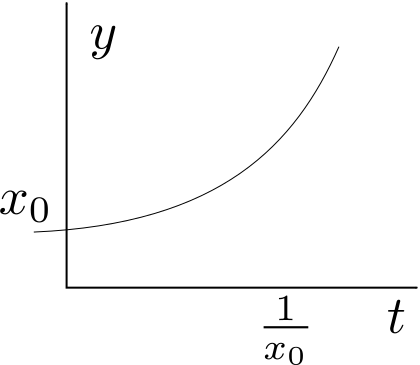
\includegraphics[width=4.5cm]{image21.pdf}
\end{figure}
\item $|s|, |t|$klein gilt:
\begin{equation*}
\varphi_{t+s}(x) = \varphi_{t}(\varphi_s(x)) \qquad 
\end{equation*}
\begin{figure}[H]
\centering
\def\svgwidth{200pt} 
  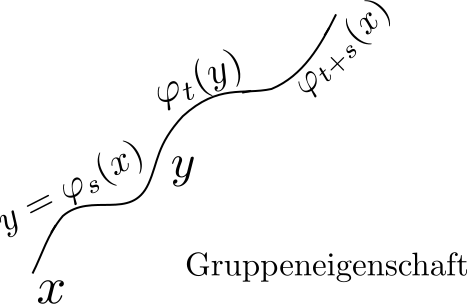
\includegraphics[width=4.5cm]{image3.pdf}
\end{figure}
Spezialfall. $s= -t:$
\begin{equation*}
\begin{matrix}
\varphi_t(\varphi_{-t}(x)) &=& \varphi_{t-t}(x)\\ 
&=&\varphi_0(x)\\ 
&=&x
\end{matrix}
\end{equation*}\\ 
$\Rightarrow \varphi_t^{-1}(x) = \varphi_{-t}(x)$
\item Ist $f$ r-mal stetig diffbar \\
$\Rightarrow \varphi$ ist $r$-mal stetig diffbar nach zustand\\ 
$\qquad \varphi$ ist $(r+1)$ mal stetig diffbar nach zeit
\item Ein Fluss, der auf $\mathrm{R}\times M$ definiert ist, heißt globaler Fluss.
\end{itemize}
\subsection*{Beispiel}
\begin{itemize}
\item Konstantes VF $f(x) = b \in \mathrm{R}^n$ \begin{equation*}
\begin{matrix}
\varphi_t(x) &=& x &+& bt \\ 
\dot \varphi_t(x)&=&b &=&f(\varphi_t(x))
\end{matrix}
\end{equation*}
\item Lineares VF $f: \mathrm{R}^n \to \mathrm{R}^n$ mit 
\end{itemize} 
Matrixexponentialfunktion: \begin{equation*}
e^A = \sum_{k=0}^{\infty} \frac{1}{k!}A^k
\end{equation*}
Gruppeneigenschaft: 
\begin{equation*}
\begin{matrix}
\varphi_t(\varphi_s(x)) &=&e^{At} e^{As} x \\ 
&=& (I + tA + \frac{1}{2} t^2 A^2 + \dots )(I + As + \frac{1}{2}A^2s^2 + \dots  )x\\ 
&=& (I + (t + s)A + \underbrace{(\frac{1}{2} t^2 + ts + \frac{1}{2} s^2 )}_{\frac{1}{2}(t+s)^2  }A^2 + \dots ) x \\ 
&=& e^{A(t+s)}x = \varphi_{t+s}(x)
\end{matrix}
\end{equation*}
\subsection*{Reihenentwicklung des Flusses}
$f: M \to \mathrm{R}^n $ glatt $\Rightarrow$ Fluss $\varphi_t$ auch glatt \\ 
Reihensatz: 
\begin{equation*}
\varphi_t(x) = v_0 (x) + v_1(x)t + v_2(x)t^2 + O(t^3)
\end{equation*}
\begin{equation*}
\text{VF} \quad v_0, v_1, v_2: M \to \mathrm{R}^n
\end{equation*}
Wegen $\varphi_0(x) \equiv x \Rightarrow v_0(x) \equiv x$ bzw. $v_0 = \text{id = Identische Abbildung}$
\\ $\Rightarrow \varphi_t(x) = x + v_1 (x)t + v_2(x)t^2 + O(t^3)  $
Einerseits: \begin{equation*} 
\begin{matrix}
f(\varphi_t(x)) &=& f(x+ v_1(x)t + v_2(x)t^2 + O(t^3)  )\\ 
&=&f(x)+ f'(x) v_1(x) t + \dots   
\end{matrix}
\end{equation*}
Anderseits: \begin{equation*}
\begin{matrix}
&\dot{\varphi}_t(x) &=& v_1(x) + 2v_2(x) t + \dots \\ 
\Rightarrow &v(x) &=& f(x)\\ 
&v_2(x) &=& \frac{1}{2}f'(x) v_1(x)
\end{matrix}
\end{equation*}
Damit \begin{equation*}
\varphi_t(x) = x + f(x) t + \frac{1}{2}f'(x) f(x)t^2 + O(t^3)\tag{2.3}
\end{equation*}
\begin{figure}[H]
\centering
\def\svgwidth{200pt} 
  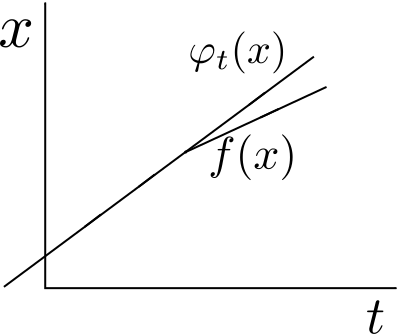
\includegraphics[width=4.5cm]{image4.pdf}
\end{figure}
Daraus folgt: 
\begin{equation*}
\frac{\partial \varphi_t(x)}{\partial x} = I + f'(x)t + \dots  \tag{2.4}
\end{equation*}
\begin{equation*}
\varphi_t(x) = x - \varphi(x) t + \frac{1}{2}f'(x) f(x) t^2 + \dots  \tag{2.5}
\end{equation*}
\subsection*{Lokale Invertierbarkeit von $\varphi_t$}
$f: M\to \mathrm{R}^n$ stetig diffbar, $p\in M$\\ $\Rightarrow$ Fluss $\varphi: I_p \times U_p \to M$
existiert und ist auch stetig diffbar.
$\varphi_t(x) = x$ \\ 
$\Rightarrow$\begin{equation*}
\varphi_0' (x) = \frac{\partial \varphi_0(x)}{\partial x} = I 
\end{equation*}ist regulär 
\\$\varphi_t'$ stetig $\Rightarrow$ für kleine $|t|$ ist auch $\varphi_t'$ regulär\\ 
Satz über Umkehrfunktion:\\ 
Es ex. offene Umgebungen $U \subset U_p$ von $p$ und $V$ von $\varphi_t(p)$, so dass $\varphi_t|_u$ (eingeschränkt auf $U$) 
bijektiv ist und eine Umkehrabb. $\varphi_t^{-1}: V\to U$, die stetig diffbar ist. \\ 
M.a.W,: $\varphi_t$ ist ein (lokale ) Diffeomorphismus
\subsection*{Satz:} Sei $\varphi_t$ der Fluss von \begin{equation*} \dot x = f(x) \tag{2.2} \end{equation*} mit stetig diffbarem VF $f: M \to \mathrm{R}^n$. Dann ist $\varphi_t'(p)$ die Lösung der Anfangswertaufgabe \begin{equation*} \begin{matrix} \dot x &=& f'(\varphi_t(p))\cdot x \\ &&x(0)=I \end{matrix} \tag{2.6} \end{equation*} Gl.(2.6) heißt Variationsgl. von (2.2). Die Lösung von (2.6) heißt (normiert)
\subsection*{Fundamentalmatrix}Beweis: Sei $\bar x(t) := \varphi_t'(p)$. 
\begin{equation*}
\begin{array}{ l l l}
\dot{\bar{x}}(t) &=& \frac{\partial }{\partial t} \bar{x}(t)\\ 
&=&\frac{\partial }{\partial t} \frac{\partial }{\partial x} \varphi_t(x)|_{x=p}\\
\text{Schwarz} &=& \frac{\partial}{\partial x} \dot{\varphi}_t (x)|_{x= p}\\ 
&=& \frac{\partial }{\partial x} f (\varphi_t (x))|_{x=p}\\ 
&=&f'(\varphi_t (x))\cdot \varphi_t'(x)|_{x=p} \\ 
&=&f'(\varphi_t(p))\cdot \bar{x}(t).
\end{array}
\end{equation*}
Das ist die AWA (2.6). \\ 
Eindeutigkeit : $x \equiv \bar{x}$. 
\chapter{Differentialgeometrische Begriffe}
\section{Differentialoperatoren}
\subsection{Lie-Ableitung eines Skalarfeldes}
Sei $M \subseteq \mathrm{R}$ offen\\ 
$f: M\to \mathrm{R}^n$ ein VF glatt\\ 
$h: M\to \mathrm{R}$ \,ein SF glatt\\ 
$\varphi_t \dots $ Fluss von $f$,\\ 
$\varphi_t(x) = x + f(x)t + \mathrm{O}(t^2)$\\ 
Lie-Ableitung des Skalarfeldes $h$ entlang des VF $f$ im Punkt $x \in M:$ 
\begin{equation*}
L_f h(x): = \frac{d}{dt} h(\varphi_t(x))|_{t=0}
\end{equation*} 
Berechnung: 
\begin{equation*}
\begin{array}{l l l}
L_f h(x) &=& \frac{d}{dt}h (\varphi_t(x))|_{t=0}\\ 
&=& \lim\limits_{t\to 0} \frac{h(\varphi_t(x)) - h\overbrace{\varphi_0(x)}^{x} }{t}\\ 
&=& \lim\limits_{t\to 0} \frac{ h(x+ f(x)t +\dots  ) - h(x) }{t}\\ 
&=&\lim\limits_{t\to 0} \frac{h(x) + h'(x) f(x)t + \dots - h(x) }{t}\\ 
&=& \lim\limits_{t\to 0} (h'(x) f(x) + \dots ) = h'(x) f(x) \\ 
&=& \langle dh(x), f(x) \rangle \\ 
&=& \sum\limits_{i=1}^{n} \frac{\partial h(x)}{\partial x_i} f_i(x).
\end{array}
\end{equation*}
\subsection*{Bemekrung:}
\begin{itemize}
\item Gemischte Lie-Ableitungen: Sei $g: M \to \mathbb{R}^{n}$ ein weiteres VF:
\begin{equation*}
L_g \underbrace{L_f h(x)}_{\text{ist SF}} = \frac{\partial L_f h(x)}{\partial x} gx
\end{equation*}
\item Mehrfache Lie-Ableitung:
\begin{equation*}
\begin{array}{ l l l}
L_f^{k+1}h(x) &=& L_f(L_f^k h(x))\\ &=& \frac{\partial L_f^{\lambda} h(x)}{\partial x}f(x)
\end{array}
\end{equation*}
\begin{equation*}
L_f^{\circ}h(x) = h(x)
\end{equation*}
Sei \begin{equation*}
\begin{matrix}
\dot x(t) &=&f(x(t))\\ 
y(t) &=&h(x(t)) 
\end{matrix}
\end{equation*}
Behauptung: 
\begin{align*}
y^{k}(t) &= L_f^k h(\varphi_t(x))\\ 
k=0: \quad y(t) &= h(x(t))
\end{align*}
\end{itemize}
\begin{equation*}
\begin{array}{l l l}
y^{k+1}(t) &=&\frac{d}{dt}y^{(k)}(t) \\ 
&=&\frac{d}{dt}L_f^{k}h(\varphi_t(x))\\ 
&=&dL_f^k h(\varphi_t(x))\cdot \dot \varphi_t(x)\\ 
&=&dL_f^k h(\varphi_t(x))\cdot f (\varphi_t(x))\\ 
&=&L_f^{k+1} h(\varphi_t(x))
\end{array}
\end{equation*}
Sei $x(0) = x_0$
\begin{align*}
\Rightarrow y^{(k+1)} (0) = L_f^{(k+1)} h(x)\\ 
\end{align*}
Sind $f,h$ analytisch $\Rightarrow$ Taylorreihe
\begin{equation*}
y(t) = \sum\limits_{k=0}^{\infty} L_f^k h(x_0)\frac{t^k}{k!} \qquad \text{Lie-Reihe}
\end{equation*}
Rechenregeln:\\  
$f, g : M \to \mathbb{R}^n \quad VF$\\ glatt
$\alpha, \beta: M\to \mathbb{R}\quad SF$ glatt
\begin{align*}
L_{\alpha \beta}\beta (x) &= \alpha(x)\cdot L_f\beta(x)\\ 
L_f(\alpha+\beta)(x)&=L_f \alpha(x) + L_f\beta(x)\\ 
* L_f(\alpha \beta)(x)&= \alpha(x) L_f\beta(x) + \beta(x) L_f\alpha(x)\\ 
L_{f+g}\alpha(x) &=L_f\alpha(x) + L_g\alpha(x)
\end{align*}
Beweis von $(*)$
\begin{align*}
L_f (\alpha \beta)(x) &= (\frac{\partial }{\partial x}(\alpha(x) \beta (x)) )\cdot f(x)\\ 
&=(\alpha(x)\beta'(x) + \beta(x)\alpha'(x) )\cdot f(x)\\ 
&=\alpha(x)\underbrace{ (\beta'(x) f(x)) }_{L_f\beta(x)} + \beta(x)(\alpha'(x)\beta(x))
\end{align*}
Ergänzung: \\ $f: M\to \mathbb{R}^n \dots VF$
$h: M\to \mathbb{R}^p \dots$ vektorrielle Abb.
\begin{align*}
h(x) &=
\begin{pmatrix}
h_1(x)\\ \vdots\\ h_p(x)
\end{pmatrix}\\
L_fh(x):&= \frac{\partial h(x)}{\partial x} f(x) = \begin{pmatrix} dh_1(x)\\\vdots\\ dh_p(x)  \end{pmatrix}f(x)\\ 
% &= \begin{pmatrix}L_fh(x)  \end{pmatrix}
\end{align*}
\begin{align*}
\begin{pmatrix}
L_f(h_1(x))\\ \vdots\\ L_fh_p(x)
\end{pmatrix}\dots \text{ vereinigte Notation für Lie-Ableitung}
\end{align*}
etwas verpasst:
\subsection{Koordinateenwechsel eines Vektorfeldes }
Seien $M, N \subseteq \mathbb{R}^n$ offen, \\ 
$\psi: M \to N\dots $Diffemorphismus 
\begin{figure}[H]
\centering
\def\svgwidth{200pt} 
  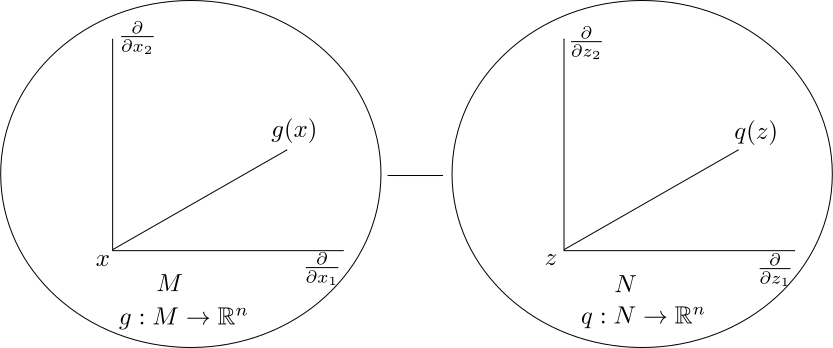
\includegraphics[width=12.5cm]{im3_12.pdf}
\end{figure}
\begin{itemize}
\item Differential, Push-Forward wird durch Jacobimatrix beschrieben $\psi_{*}(x) = \psi'(x) $
\item Rücktranspormation, Push-Back: 
\begin{align*}
\psi^{*} (z):&= \psi_{*}^{-1} (z)\\ 
&=(\psi^{-1})' (\underbrace{\psi(x)}_{z})\\ 
&=(\psi' (x))^{-1}   
\end{align*}
\item Push-Forward: 
\begin{align*}
\dot z &= \frac{d}{dz}  z  = \frac{d}{dt} \psi (x)\\ 
&= \psi'(x)\dot x\\ 
&= \psi'(x)g(x)\\ 
&= \psi_{*}g(x)|_{x=\psi^{-1}(z)}\\ 
&= \underbrace{\psi_{*}g(\psi^{-1} (z))}_{q(z)}
\end{align*}
\subsection*{Beispiel}lin. VF: $g(x) = Ax$\\ lin. Transf: $z= Tx$\\ 
$\dot z = T\dot x= TAx = TAT^{-1} z$ Ähnlichkeitstrans.\\ 
Rücktransform. und Pull-Back: 
\begin{align*}
\dot x = \frac{d}{dt}x &= \frac{d}{dt}\psi^{-1}(z) = (\psi'(z))^{-1}\dot z\\ 
&=(\psi'(z))^{-1}q(z)\\ 
&=\psi_{*}^{-1}q (\psi(x))=\underbrace{\psi^{*} q(z)}_{g(x)}
\end{align*}
\begin{figure}[H]
\centering
\def\svgwidth{200pt} 
  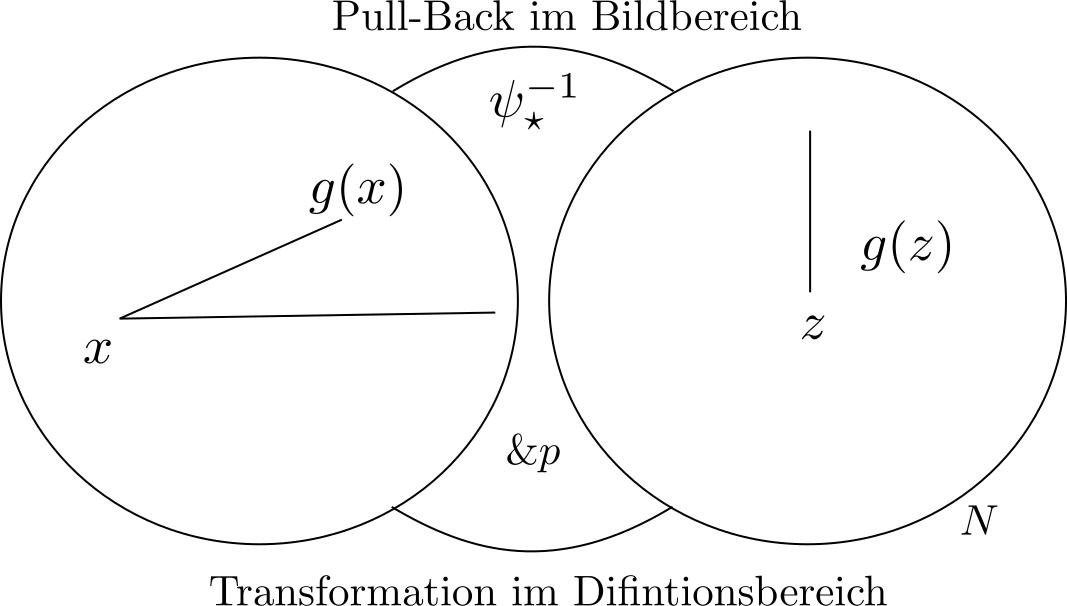
\includegraphics[width=7.5cm]{im3_121.pdf}
\end{figure}
\end{itemize}
\subsection{Lie-Ableitung eines Vektorfeldes}
Spezialfall: $\psi = \varphi_t,$ d.h. der Diffeomorphismus ist Fluss eines VF $f$ zu Zeit $t$ 
\begin{figure}[H]
\centering
\def\svgwidth{200pt} 
  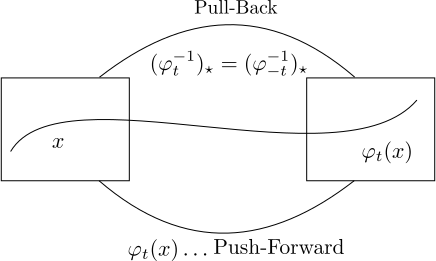
\includegraphics[width=7.5cm]{im3122.pdf}
\end{figure}
Reihenentwicklungen:
\begin{align*}
\psi_{t*}(x) &= I + f'(x)t + O(t^2)\\ 
\psi_{t*}(x) &= I- f'(x) + O(t^2)
\end{align*}
Lie - Ableitung bzw. Lie-Klammer eines VF $g: M\to \mathbb{R}^n$ entlang $f:$
\begin{align*}
[ f,g](x) = L_fg(x) := \frac{d}{dt}\underbrace{\varphi_{-t*}g(\varphi_t(x))}_{Ad_{t,f}g(x)}|_{t=0}\\ 
\end{align*}
Zeitinvarinater Operator für VF\\ 
\begin{align*}
Ad_{t,f}g(x)&=\varphi_{-t}'(z) g(z)|_{z=\varphi_t(x)}\\ 
&=(I - f'(z)t+ O(t^2))\cdot g(z)|_{z= x+ f'(x)t+ O(t^2)}\\ 
&=(I - f'(x)t+ O(t^2))\cdot \underbrace{g(x+ f(x)t + O(t^2) ) }_{g(x) + g'(x)f(x)t+ O(t^2) }\\ 
&=g(x) + \underbrace{g'(x)f(x) - f'(x)g(x) }_{[f,g](x)}t + O(t^2)
\end{align*}
\subsection*{Beispiel}
Lineares VF $f(x) = Ax,\qquad A\in \mathbb{R}^{n\times n}$\\
Konstan. VF $g(x) = b \in \mathbb{R}^n$
\begin{align*}
[f,g] &= \underbrace{g'}_{\equiv 0} f - f'g = -Ab = ad_f g\\ 
\Rightarrow [-f,g]_{\text{Def.}} &= ad_{-f}g = Ab\\ 
&\Rightarrow ad_{-f}^{k}g = A^k b
\end{align*}
Koordninationtransf: Sei $\psi. M \to N$ ein Diffeomorphismus. Dann gilt 
\begin{align*}
\psi_*[f,g] = [\psi_*f, \psi_* g]
\end{align*}
Weitere Rechenregeln: 
\begin{align*}
f,g : M\to \mathbb{R}^{n} &\qquad \text{VF}\\ 
\alpha, \beta: M\to \mathbb{R}&\qquad \text{SF}\\ 
&\\
L_{[f,g]} \alpha(x) &= L_f L_g \alpha(x) - L_gL_f\alpha(x)\\ 
[\alpha f,\beta g] (x) &= \alpha(x)\beta(x) [f,g](x) + \alpha(x)L_f\beta(x)\cdot g(x) - \beta(x)L_g \alpha(x)g(x)
\end{align*}
Beweis von $(*)$: 
\begin{align*}
L_g L_f\alpha(x) &= dL_f\alpha(x)\cdot g(x)\\ 
&= (\alpha'(x)f'(x) ) + f^T (x) \alpha'' (x) g(x) \tag{1}\\ 
\Rightarrow L_f L_g\alpha(x)&=(\alpha (x) g'(x) + g^T(x) \alpha'' (x) )\cdot f(x) \tag{2} \\ 
(2)-(1) &= \alpha'(x) (g'(x)f(x) - f'(x)g(x) )\\ 
&=\alpha'(x) [f,g] (x) = L_{[f,g]}\alpha(x)
\end{align*}
Interpretation : (+) ist Differeantialoperator 1. Ordnung
\subsection*{Bemerkung}
\begin{itemize}
\item Mehrfache Lie-Klammer entlang gleichem VF 
\begin{align*} 
ad_{f}^{k+1} g(x) &:= [f, ad_{f}^{k}g ] (x) \\
ad_{f}^{0}g(x) &:= g(x)\\ 
\underbrace{[f,[f,\dots,[f,g]\dots ]]}_{\text{k mal}} &:= ad_f^h g(x)
\end{align*}
\item Zwei lineare VF
\begin{align*}
f(x)&=A\,x\\ 
g(x)&=B\,x, \qquad A B \in \mathbb{R}^{n\times 1}\\ 
[f,g](x)&=(g'f - f'g)(x)\\ 
&=\underbrace{(BA - AB)}_{\text{Kommutator}}(x)
\end{align*}
\end{itemize}
\subsection*{Beispiel} Mobiler Roboter
\begin{align*}
\begin{pmatrix}
\dot x_1\\ \dot x_2\\ \dot x_3 
\end{pmatrix} = 
\underbrace{
\begin{pmatrix}
\sin{x_3}\\ \cos{x_3}\\ 0 
\end{pmatrix}}_{f(x) \text{ transl. Teil}} u_1 + \underbrace{
\begin{pmatrix} 0\\ 0\\ 1 
\end{pmatrix}}_{g(x)\text{ rot. Teil}} u_2
\end{align*}
\begin{align*}
[f,g]= \underbrace{g'f}_{O \in \mathbb{R}^{3\times 3}} - f'g = -f'g = \begin{pmatrix} 0 & 0 & \cos{x_3}\\ 0&0&-\sin{x_3}\\ 0&0&0\end{pmatrix} \begin{pmatrix} 0\\ 0\\ 1\end{pmatrix} = \begin{pmatrix} \cos{x_3}\\ -\sin{x_3}\\ 0 \end{pmatrix}
\end{align*}
\subsection{Pull-Back und Lie-Ableitung eines Kovektorfeldes}
$\psi \dots$ Diffeomorphismus\\ 
$\psi_{*} = \psi' \dots $ Push-Forward für ein Vektorfeld\\ 
$\omega \dots $ KVF \\ 
zu $\psi_{*}$ gehörende duale oder adjungierte Abbildung $\psi^{*}$ ist definiert durch \begin{equation*}< \psi^* \, \omega \, f> = <\omega, \psi, f> \tag{*} \end{equation*} $\Rightarrow$ Pull-Back - Abb. des KVF $\omega$
\begin{equation*}
\underbrace{y^T}_{\text{Zeilenvektor}} \cdot (\underbrace{A}_{\text{Spaltenvektor}}x) = y^T \cdot A\cdot x = (\underbrace{A^T y}_{\text{Zeile}})^T \cdot \underbrace{x}_{\text{Spalte}}
\end{equation*}
Spezialfall: $\psi = \varphi_t$, d.h. Diffeomorphismus ist Fluss des VF $f.$
\begin{align*}
\varphi_t^{*} \omega(x) &\underset{*}{=}  \omega(x) \varphi_{t*}\\ 
&= \omega (x) (I + f'(x)t + O(t^2))
\end{align*}
Lie-Ableitung eines Kovektorfeldes
$\omega : \mathbb{M} \to (\mathbb{R})^* $ entlang $f$: 
\begin{align*}
L_f \omega(x) = \frac{d}{dt}\underbrace{\varphi_t^* \omega (\varphi_t (x))}_{=: Ad_{t,f} \omega(x)}\Big|_{t=0}
\end{align*}
Reihenentwicklung: 
\begin{align*}
Ad_{t,f} \omega(x) &\underset{\text{Def}}{=} \varphi_t^* \omega(\varphi_t (x))\\ 
&\underset{(*)}{=} \omega (z) \varphi_t' (z)\Big|_{z=\varphi_t(x)}\\ 
&\underset{(*)}{=} \omega \left( x + f(x)t + \dots \right) \left( I + f'(x) t + \dots \right)\\ 
&=\left( \omega (x) + f^T (x)\left(\frac{\partial \omega^T}{\partial x}\right)^T + \hdots \right)\left( I + f'(x)t + \hdots \right)\\
&=\omega(x) + \underbrace{\left( f^T (x)\left(\frac{\partial \omega^T}{\partial x}\right)^T + \omega(x)f'(x) \right)}_{L_f \omega(x)}t + \dots
\end{align*}
Rechenregeln 
\begin{align*}
f,g &\dots VF\\ 
\omega &\dots KVF\\ 
\alpha&\dots SF
\end{align*}
\begin{enumerate}[(a)]
\item $L_f d \alpha = d L_f \alpha$
\item \begin{align*}L_f < \omega, g>(x) &= <L_f \omega, g>(x) + <\omega, [f,g]> (x)\\ 
\text{Beweis: a). } dL_f \alpha(x) &= \frac{\partial }{\partial x}L_f \alpha(x)\\ 
&= \frac{\partial}{\partial x}(\alpha' (x) f(x))\\ 
&= (\alpha'(x) f'(x) + f^T (x) \alpha''(x))\\ 
&= \alpha'(x) f'(x) + f^T (x) \left( \frac{\partial (\alpha'(x))^T}{\partial x} \right)^T\\ 
&= L_f\alpha(x)
\end{align*}
\end{enumerate}
\section{Lie-Klammer und dynamische Systeme}
\subsection*{Lemma:} Seien $\varphi^f, \varphi^g$ die Fläche des VF $f,g$. Die Flüße kommutieren genau dann, wenn die Lie-Klammer der Vektorfeldes identisch Null ist. 
\begin{align*}
\varphi_t^f\cdot \varphi_s^g = \varphi_s^g \cdot \varphi_t^f \iff [f,g] = 0
\end{align*}
Beweis: $\Rightarrow$
\begin{align*}
\varphi_s^g (\varphi_t^f(x)) &= \varphi_s^g \overbrace{(x + f(x)t + \dots)}^{z} \\ 
&= \underbrace{x + f(x)}_{z} t + \underbrace{g(x + f(x)t+ \dots)}_{g(z)s}s + \dots\\ 
&= x+ f(x)t + g(x)s + g'(x)f(x)st + \dots\\ 
\varphi_t^f(\varphi_s^g(x))&=x+ g(x)s + f(x)t + f'(x)g(x)ts + \dots\\ 
\overset{\text{Differenz:}}{\varphi_s^g(\varphi_t^f(x))}&- \varphi_t^f(\varphi_s^g(x)) = \underbrace{(g'(x)f(x) - f'(x)g(x)}_{[f,g]}st+ \dots )
\end{align*}
Differenz ist 1t. Annahme die Nullfunktion\\ 
$\Rightarrow $ alle Koeff. einer Reihenentwicklung und identisch Null insbesondere $[f,g]\equiv 0$.\\ 
Anwendung auf lineare VF
\begin{align*}
f(x)&= A\,x \\ 
g(x)&= B\,x \\
\end{align*}
$e^{At}\cdot e^{Bs} = e^{Bs} \cdot e^{At}$
$\iff [A,B] = 0$ d.h. $BA - BA = 0$\\ 
$\iff AB = BA$\\ 
System mit 2 Eingängen: 
\begin{equation*}
\dot x = f(x)u_1 + g(x)u_2
\end{equation*}
Zwischen den VF $f,g$ wird mittels $u_1,u_2$ nach folgenden Schema umgeschaltet\\  \\
\begin{tabular}{c | c | c | c }
Schritt & $u_1$ & $u_2$ & $f_1 u_1 + g u_2$ \\ 
\hline
1 & 1 & 0 & f \\ 
2 & 0 & 1 & g \\ 
3 & -1& 0 & -f\\ 
4 & 0 &-1 & -g
\end{tabular}\\ 
Darstellung 
\begin{equation*}\gamma(t) := \varphi_t^{-g} \cdot \varphi_t^{-f} \cdot \varphi_t^g \cdot \varphi_t^f(x) \end{equation*} 
Mit Reihenentwicklung der Flusses erfüllt man 
\begin{align*}
\gamma(t) = x + \underbrace{(g'(x)f(x) - f'(x)g(x) )}_{[f,g]}t^2 + \dots
\end{align*}
\begin{figure}[H]
\centering
\def\svgwidth{200pt} 
  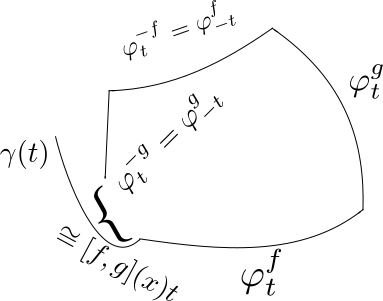
\includegraphics[width=6.5cm]{image332.pdf}
\end{figure}
\begin{align*}
\gamma(\sqrt{t}) &= x + [f,g](x)t + \dots\\ 
& \approx \varphi_t^{[f,g]} (x) 
\end{align*}
\subsection*{Beispiel}
Robotermodell
\begin{align*}
f(x) = \begin{pmatrix} \sin{x_3} \\ \cos{x_3}\\ 0 \end{pmatrix}, \qquad g(x) = \begin{pmatrix} 0\\ 0\\ 1\end{pmatrix} \\ 
[f,g](x) = \begin{pmatrix} -\cos{x_3}\\ \sin{x_3}\\ 0 \end{pmatrix}
\end{align*}
\begin{figure}[H]
\centering
\def\svgwidth{200pt} 
  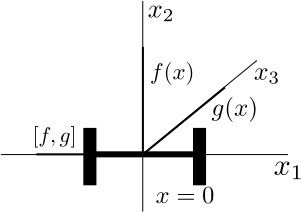
\includegraphics[width=6.5cm]{robmod1.pdf}
\end{figure}
Mittelung des Systems 
\begin{align*}
\dot x = f(x)\cdot u_1(t) + g(x)\cdot u_2(t) \qquad \text{ mit } &u_1(t)= \sqrt{\omega}\cdot \cos{(\omega t)}\\ 
&u_2(t) = \sqrt{\omega}\cdot \sin{(\omega t)}, \omega > 0
\end{align*}
führt für $\omega \to \infty$ auf $\dot x^\infty = \frac{1}{2} [f,g] (x^\infty)$
\section{Distributionen und Kodistributionen}
$M \in \mathrm{R}^n$ offen, $f_1, \dots, f_r : M\to \mathbb{R}^n \dots $ glatte VF. in jedem Punkt $x\in M $ spannen die VF einen UVR des $\mathbb{R}^n$ auf $\text{span}\{ f_1(x),\dots, f_r(x)\}$ \\ 
Die Zuordnung \begin{align*}
M \ni x \to \Delta(x) = \underbrace{\text{span}\{ f_1(x),\dots,f_r(x) \}}_{\in \mathbb{R}^n}
\end{align*}
heißt Distribution.\\ 
Glatte Distribution wird von glatten VF aufgespannt.\\ 
Punktweise Überlagerung von Operation auf UVR auf Distributionen. 
\begin{itemize}
\item Summe: $(\Delta_1 + \Delta_2)(x) = \Delta_1(x)  + \Delta_2(x)$
\item Durchschnitt: $(\Delta_1 \cap \Delta_2)(x) = \Delta_1(x) \cap \Delta_2(x)$
\item $f \in \Delta: \iff \forall x\in M: f(x) \in \Delta(x)$
\item $\Delta_1 \le \Delta_2 \iff \forall x\in M : \Delta_1(x) \le \Delta_2(x)$\\ 
\end{itemize}
VF zu Matrix zusammenfassen: 
\begin{align*}
F(x) &= (f_1(x),\dots, f_r(x))\\ 
\text{im}F(x) &= \text{span}\{ f_1(x),\dots,f_r(x) \}\\ 
&=\Delta(x)
\end{align*}
$\Delta$ heißt regulär (im Punkt $x_0 \in M$)\\ 
$\exists r \in \mathbb{N}_0: \text{dim}\Delta(x) = r$ für alle $x$ aus Umgebung von $x_0$
\subsection*{Beispiel}
$f_1(x) = \begin{pmatrix} \cos{x_3}\\ \sin{x_3} \\ 0 \end{pmatrix}, f_2(x) = \begin{pmatrix} -\sin{x_3}\\ \cos{x_3}\\ 0 \end{pmatrix}$\\ 
\begin{align*}F(x) &= (f_1(x), f_2(x)) \\
&= \begin{pmatrix}
\cos{x_3} & -\sin{x_3}\\ \sin{x_3} & \cos{x_3}\\ 0& 0
\end{pmatrix}\\
\Delta(x)&= \text{span}\{ f_1(x), f_2(x) \}\\ 
&= \text{im}F(x) \\ 
&= \text{span}\{e_1,e_2\} = \text{im}\begin{pmatrix} 1&0\\ 0&1\\ 0&0 \end{pmatrix} 
\end{align*}
\subsection*{Lemma 3.1:} $\Delta \dots$ glatte Distribution, regulär im Punkt $x_0 \in M$ mit Dimension $r$. \\ 
Dann existiert Umgebung $U\in M$ von $x_0$ und $r$ VF $f_1, \dots, f_r: U\to \mathbb{R}^n$, so dass für alle $x \in U$ gilt. 
\begin{enumerate}
\item Die Vektoren $f_1(x), \dots, f_r(x)$ sind linear unabhängig. 
\item $\Delta(x) = \text{span}\{ f_1(x), \dots, f_r(x) \}$\\ 
Jedes VF $f\in \Delta$ kann auf $U$ wie folgt dargestellt werden. \begin{align*} f(x) = \sum\limits_{i=1}^r \alpha_i(x) f_i(x) \end{align*} mit glatten SF $\alpha_1,\dots,\alpha_r: U\to \mathbb{R}^n$\\
$f_i\dots$ Basisvektorfelder
\end{enumerate}
Berechnung der SF: Lineare Gleichung
\begin{align*}
\underbrace{(f_1(x), \dots, f_r(x))}_{F(x)} \underbrace{\begin{pmatrix} \alpha_1(x)\\ \vdots\\ \alpha_r(x) \end{pmatrix}}_{\alpha(x)}= f(x)
\end{align*}
$\omega_1,\dots, \omega_r : M \to (\mathbb{R}^n)^*\dots $KVF\\ 
Diese spannen im Dualraum $(\mathbb{R}^n)^*$ eine Kodistribution auf \begin{align*} \Omega = \text{span}\{\omega_1,\dots, \omega_r\} \end{align*}
Annihilator $\Delta^\perp$ eine Distribution $\Delta:$ 
\begin{align*}
\Delta^{\perp}(x) = \{ \omega_1 \in (\mathbb{R}^n)^*: \langle \omega, v \rangle = 0 \text{ für alle } v\in \Delta(x) \}
\end{align*}
Annihilator $\Omega^{\perp}$ eine Kodistribution: $\Omega^\perp  = \{ v\in \mathbb{R}^n: \langle \omega, v \rangle = 0 \text{ für alle } \omega \in \Omega(x) \}$
\subsection*{Beispiel}
$\Delta(x) = \text{span}\left\{ \begin{pmatrix} 1\\ 0\\ 0 \end{pmatrix}, \begin{pmatrix} 0\\ e^{x_3}\\ 0 \end{pmatrix} \right\}$
\begin{align*}
\Delta^\perp (x)&= \text{span}\{ (0, 0, 1) \}\\ 
F(x) &= (f_1(x), \dots, f_r(x))\\ 
w(x) &= \begin{pmatrix} \omega_1(x)\\ \vdots\\ \omega_r(x) \end{pmatrix}
\end{align*}
\begin{itemize}
\item $\Delta^\perp(x) $ aufgespannt von KVF $\omega$ mit $\omega(x) \cdot F(x) = 0 \in (\mathbb{R}^r)^*\qquad (0) $
\item $\Omega^\perp(x) $ wird aufgespannt von VF $v$ mit $\omega(x)\cdot v(x) = 0 \in \mathbb{R}^x$\\ letztes ist der Kern von $\omega:$ \begin{align*}
\Omega^{\perp} = \text{ker} \,\omega(x) \end{align*}
\item Transfonieren von $(0)$ liefert $\Delta^\perp (x) = (\text{ker} \,F^T (x))^T$
\end{itemize}
Bemerkung: Seien $\Delta, \Delta_1, \Delta_2$ Distribution
\begin{itemize}
\item $\text{dim}(\Delta) + \text{dim}(\Delta^\perp) = n $
\item $\Delta_1 \le \Delta_2 \iff \Delta_1^\perp \ge \Delta_2^\perp $
\item $(\Delta_1 \cap \Delta_2)^\perp = \Delta_1^\perp + \Delta_2^\perp $
\end{itemize}
\section{Involitive Distributionen}
\subsection*{Defintion:} Sei $f: M\to \mathbb{R}^n$ lineare VF. Eine Distribution $\Delta$ heißt invariant unter elem. VF $f(f\to \text{invariant})$, wenn $\forall g\in \Delta$: $[f,g]\in \Delta$. Eine Distribution ist involitiv, wenn sie für jedes der VF invariant ist. 
\subsection*{Definition:}Eine Distribution $\Delta$ heißt involitiv, wenn 
\begin{align*}
\forall f,g \in \Delta: [f,g] \in \Delta \tag{A}
\end{align*}
\subsection*{Lemma 3.2:} Sei $\Delta = \text{span}\{f_1,\dots, f_r\},\qquad \Delta $ genau dann involitiv, wenn \begin{align*}
[f_i,g_j] \in \Delta f \quad i\le j , j\le r \tag{B}
\end{align*}
\subsection*{Beweis}
\subsection*{$\Rightarrow$}
 $\Delta$ sei involitiv, d.h. $(A)$ gilt für alle VF von $\Delta$. Dann gilt $(A)$ auch für die VF $f_1,\dots, f_r$, d.h $(B)$ ist erfüllt. 
\subsection*{$\Leftarrow$} Es gilt $(B)$. Für $f,g \in \Delta $ gibt es SF $\alpha_1,\dots,\alpha_r$ und $\beta_1,\dots,\beta_r$ mit
\begin{align*}
f(x) &=\sum\limits_{i=1}^{r} \alpha_i (x)f_i(x) \\ 
g(x) &=\sum\limits_{i=1}^{r} \beta_i(x)\cdot f_i(x)
\end{align*}
Rechenregeln für Lie-Klammer liefern. 
\begin{align*}
[f,g] &= \left[ \sum\limits_{i=1}^{r} \alpha_i f_i, \sum\limits_{j=1}^{r} \beta_j f_j \right]\\ 
&= \sum\limits_{i=1}^{r}\sum\limits_{j=1}^r\left\{ \alpha_i \beta_j [f_i, \beta_j] + \alpha_i (L_{f_i} \beta_j)f_j - \beta_j(L_{f_j} \alpha)f_i \right\}
\end{align*}
$\Rightarrow [f,g] = \underbrace{\text{span}\{ f_1, \dots, f_r \}}_{=\Delta} + \underbrace{\text{span}\{ f_i, f_j ]; 1\le i, j\le r \}}_{\le \Delta \text{ wegen } (B)} = \Delta$
Also gilt $(A)$
\begin{align*}
(\alpha(x)\cdot f(x))' &= \alpha(x)\cdot f'(x) + f(x)\cdot \alpha'(x)\\ 
(\beta(x)\cdot g(x))' &= \beta(x)\cdot g'(x) + g(x)\cdot \beta'(x) \\ 
\Rightarrow [\alpha f, \beta g] &= (\beta g)'\alpha f - (\alpha f)' \beta g \\ 
&= \beta g'\alpha f + g \beta'\alpha f - \alpha f' \beta g -f \alpha'\beta g \\ 
&= \alpha \beta \underbrace{(g'f - f'g)}_{[f,g]} + \alpha \underbrace{\langle d \beta, f \rangle}_{L_f \beta} g - \beta \underbrace{\langle d \alpha, g \rangle}_{L_g \alpha} f 
\end{align*}
\subsection*{Lemma 3.3:}
Die Distribution $\Delta$ sei involitiv und im Punkt $x_0 \in M$ regulär $(M \le \mathbb{R}^n, \text{ offen }).$ Dann existiert eine Umgebung $U \le M$ von $x_0$ und VF $g_1, \dots, g_r: \quad U\to \mathbb{R}^n$ mit \begin{align*} \Delta|_{n} = \text{span}\{ g_1,\dots, g_r\} \qquad \text{und } \forall x\in U: [g_i, g_j] = 0 \text{ für } 1\le i, j\le r \end{align*} 
\subsection*{Beweis:} Sei $r = \text{dim } \Delta(x_0).$ Dann $\exists r$ linear unabhängige VF $f_1,\dots, f_r$ die (lokeal) $\Delta$ aufspannen $n\times r$-Matrix \begin{align*} F(x) = (f_1(x), \dots, f_r(x)) \end{align*} 
\\$\Rightarrow$: $\Delta = \text{im }F(x)$ und $\text{rang }F(x) = r$ \\ 
$\Rightarrow: \exists r\times r $ Teilmatrix $B(x)$ von $F(x)$, die regulär ist. Ohne Einschränkung\footnote{O.E =Ohne Einschränkung} setze sich $B$ aus den $r$ Zeilen zusammen. \footnote{O.B.d.A = Ohne Beschränkung der Allgemein}\\ 
Rechtsmultiplikation mit $B^{-1}$ möglich: $\Rightarrow$ def. damit VF $g_1,\dots, g_r$ \begin{align*} F(x)\cdot B^{-1} = \left(\frac{B(x)}{*}\right)\cdot B^{-1}(x) = \left(\frac{I_r}{*}\right) =:(g_1(x),\dots,g_r(x))\\ 
\Delta = \text{span}\{ f_1,\dots,f_r \} = \text{im }F = \text{im }(F\cdot B^{-1}) = \text{span }\{g_1,\dots, g_r \}\end{align*}
Zusätzlich ist $\Delta$ involutiv, d.h. Es gilt SF $\alpha_1,\dots,\alpha_r$ mit $[g_i,g_j](x) = \alpha_1(x) g_1(x) + \dots + \underbrace{\alpha_r(x)\cdot g_r(x)}_{\text{Lemma 3.2}}$
Spezielle Form der VF $g_i, g_j:$
\begin{align*}
\begin{pmatrix} 0\\0\\ \vdots \\ 0\\ \star \end{pmatrix} = \alpha_1(x)\begin{pmatrix} 1\\ 0\\ \vdots\\ 0\\\star\end{pmatrix} + \dots + \alpha_r(x)\begin{pmatrix}0\\ \vdots\\ 0\\1\\\star\end{pmatrix}
\end{align*}
Vergleich der ersten $r$ Zeilen 
\begin{align*}
\Rightarrow& \qquad \alpha_1 \equiv \dots \equiv \alpha_r \equiv 0\\
\Rightarrow& \qquad [g_i,g_j] \equiv 0
 \end{align*}
 Satz über die simultane Begründung von VF: Sei $x_0 \in M.$ Für alle VF $f_1,\dots, f_r: M\to \mathbb{R}^{n}$ gelte. 
 \begin{enumerate}
\item $f_1(x),\dots, f_r(x)$ und linear unabhängig
\item $[f_i, f_j](x) = 0, \quad 1\le i\le r \dots$ für alle $x$ aus Umgebung von $x_0$. Dann existiert ein lokale Diffeomorphismus $z= T(x)$ und $T(x_0) = 0,$ so dass \begin{align*} = \left.\frac{T_+ f_i(x)}{T'(x)f_i(x)}\right|_{x=T^{-1}(z)} = \frac{\partial}{\partial z_i} = e_i,\qquad 1\le i \le r \end{align*}
für alle $z$ aus einer Umgebung der Null. 
\end{enumerate}
\subsection*{Beweis:}
Dann existiert $n-r$ welche VF $f_{r+1},\dots, f_n : \quad U\to \mathbb{R}^n \qquad (U\le M, \text{ Umgebung von } x_0)$. So dass $f_1,\dots, f_n$ in $U$ linearunabhängig sind. 
\subsection*{Abbildung $S$} $x = S(z):=\varphi_{z_1}^{f_1} \circ \dots \circ \varphi_{z_n}^{f_n}(x_0)$ \\ 
Reihenentwicklung nach $z$: \begin{align*} x = x_0 + f_1(x_0) z_1 + \dots + f_n(x_0)z_n + O(\|z\|)^2. \qquad \varphi_t^f(x) = x+ f(x)t + O(t^2)\end{align*}
\\Jacobi-Matrix: \begin{align*} S'(x) = \left( \underbrace{f_1(x_0),\dots, f_n(x_0)}_{\text{linear unabhängig, }S'(0) regulär} \right)\in \mathbb{R}^{n\times n} \end{align*}
Satz über Umkehrfunktion $\to$ $S$ ist ein (lokaler) Diffeomorphismus mit Umkehrabbildung $z = T(x).$\\ 
Wegen Bedingung 2 gilt für $i = 1 \dots r$ \begin{align*} S'(z)\underbrace{\frac{d}{dz_i}}_{e_i} &= \frac{\partial}{\partial z_i}S(z)\\ &=\frac{\partial}{\partial z_i} \varphi_{z_1}^{f_1} \circ \dots \circ \varphi_{z_i}^{f_i} \circ \dots \circ \varphi_{z_n}^{f_n}(x_n)\\ &=\frac{\partial}{\partial z_i}\varphi_{z_i}^{f_i} \circ \varphi_{z_1}^{f_i} \circ \dots \circ \varphi_{z_n}^{f_n}(x_0) \\ &=f_i \left( \varphi_{z_1}^{f_1}\circ \dots \circ \varphi_{z_n}^{f_n}(x_0) \right)\\ &=f_i\left.\left( S(z) \right) = f_i(x)\right|_{x= S(z)}  \end{align*}
Damit 
\begin{align*} S'(z) = \frac{\partial}{\partial z_i} =\left. f_i(x)\right|_{x= S(z)} \overset{\substack{S = T^{-1}\\ T = S^{-1}}}{\iff} \frac{\partial}{\partial z_i} = \left.T'(x)f(x)\right|_{x = T^{-1}(z)} \end{align*}
Folgerung (Begradigung von Nichtruhelagen)\\ 
Sei $x_0\in M: f: M\to \mathbb{R}^n$ ein VF mit $f(x_0)\ne 0$ (keine Ruhelagen)\\ 
Dann existiert lokaler Diffeomorphismus $z = T(x)$. \begin{align*} T'(x) f(x)|_{x = T^{-1}(z)} = \frac{\partial}{\partial z_1} = e_i \end{align*}
\begin{figure}[H]
\centering
\def\svgwidth{200pt} 
  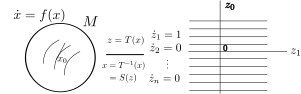
\includegraphics[width=8.5cm]{Zeichnung1.pdf}
\end{figure}
\subsection*{Definition:} Eine reguläre Distribution $\Delta$ mit $\text{dim }\Delta = r$ heißt integrierbar, wenn es SF $\lambda_1, \dots, \lambda_{n-r}$ gibt, so dass $\Delta^{\perp} = \text{span }\{d \lambda_1,\dots, d\lambda_{n-r}\}$. 
\subsection*{Satz von Frobenius:} Die Distribution $\Delta$ sei im Punkt $x_0$ regulär. Dann gilt $\Delta$ ist involutiv $\iff$ $\Delta$ ist integrierbar.
\subsection*{Beweis (lokal):} $\Delta$ regulär $\Rightarrow \exists r$ linear unabhängige VF $f_1, \dots, f_r$ mit $\Delta = \text{span }\{ f_1, \dots, f_r\}$\\ 
$\Rightarrow$ Sei $\Delta $ involutiv $\underset{\text{Lemma 3.3}}{\Rightarrow}$ die VF können so gewählt werden, dass $[f_i, f_j] = 0$ für $1\le i, j\le r_i$ 
\subsection*{Begradigungssatz:} $\exists$ lokaler Diffeomorphismus \begin{align*} T = \begin{pmatrix} t_1 \\ \vdots\\ t_n \end{pmatrix} \end{align*} mit 
\begin{align*} T'(x) f_i(x)|_{x = T^{-1}(z)} = \frac{\partial}{\partial z_i} = e_i \text{ für } i= 1,\dots,r\end{align*}  \\ wodurch VF $f_1,\dots, f_r$ in Richtung der Einheitsvektoren $\frac{\partial}{\partial z_1} ,\dots,\frac{\partial}{\partial z_r}  $ ausgerichtet werden.
Die Kovektoren $d z_{r+1} = e_{r+1}^T ,\dots, d z_{n} = e_{n}^T$ der dualen Basis. \\ Sind dann orthogonal: \begin{align*} \langle \underbrace{d z_j}_{e_j^T}, \underbrace{\frac{\partial}{\partial z_i}}_{e_i} \rangle = 0 \qquad \substack{i = 1, \dots, r\\ j = r+1, \dots, n} \end{align*}
\begin{align*}
\Rightarrow 0 &= \langle d z_j, \frac{\partial}{\partial z_i} \rangle = \langle d z_j , T'(x) f_i(x) \rangle \\ 
&= \langle \underbrace{dz_j}_{e_j^T} T'(x), f_i(x) \rangle = \langle d t_j (x), f_i(x) \rangle
\end{align*}
Die KVF $dt_{r+1}, \dots, dt_n$ sind orthogonal zu den VF, die $\Delta$ aufspannen, also sind sie im Annihilator. \\ 
$T$ ist Diffeomorphismus \begin{align*}&\Rightarrow T'(x) \text{ ist regulär} \\ &\Rightarrow \text{ Zeilenvektoren } dt_i \text{ sind linear unabhängig} \end{align*}  
$\lambda_k = t_{r+k} $ für $k= 1, \dots, n-r$\\ 
$\iff 0 = \langle d \lambda_j, f_i(x) \rangle = 0$\\ 
$\iff \lambda^{\perp} = \text{span }\{ d\lambda_1,\dots,d\lambda_r \}.$
\subsection*{Definition:} Die kleinste involutive Distribution , die $\Delta$ enthält, heißt involutive Abschluß von $\Delta : \text{inv} (\Delta)$ .
\chapter{übersprungen}
\chapter{Reglerentwurf mittels exakter Linearisierung}
\section{Eingangs-Ausgangs-Linearisierung eingangsaffiner Systeme}
\subsection{Relativer Grad und grundsätzliches Vorgehen}
Eingangsaffines System \begin{align*}
\dot x &= f(x) + g(x)\cdot u \\ 
y &= h(x) \tag{5.1}
\end{align*}
mit \begin{align*} 
&\text{VF} \quad  f,g:M\to \mathbb{R}^n\\
&\text{SF} \quad \quad h  :M\to \mathbb{R}\\
M\le \mathbb{R}^n,& \text{ offen}
\end{align*}
Zeitableitungen des Ausgangs: \begin{align*} \dot y(t) &= \left.\frac{d}{dt} h(x(t))\right|_{(5.1)}\\ 
&=h'(t)\cdot \dot x\\ 
&=h'(t)\cdot (f(x) + g(x) \cdot u)\\ 
&=L_fh(x) + L_gh(x)\cdot u 
\end{align*}
Falls $L_gh(x) \ne 0: $ STOP\\ 
Falls $L_gh(x) \equiv 0,$\\$\dot y$ hängt nicht explizit von $u$ ab.\\ 
Zweite Zeitableitung des Ausgangs:
\begin{align*}
\ddot y(t) &= \frac{d}{dt} L_fh(x(t))\\ 
&=dL_fh(x)\cdot \underbrace{(f(x) + g(x)\cdot u)}_{\dot x}\\ 
&=L_f^2h(x)\cdot(L_gL_f h(x))\cdot u
\end{align*}
\subsection*{Definition 5.1:} System (5.1) hat im Punkt $p\in M$ den \textbf{relativen Grad} $r$, wenn 
\begin{enumerate}
\item $L_g L_f^k h(x) = 0\quad $ für $k= 0, \dots, r-2$\\ und alle $x$ aus offener Umgebung von $p$.
\item $L_g L_f^{r-1} h(p) \ne 0$. 
\end{enumerate}
Interpretation: Relativer Grad ist niedrigste Ordnung einer Zeitableitung des Ausgangs von $(5.1)$, die explizit vom Eingang $u$ abhängt.\\ 
\subsection*{Reglerentwurf (allg. Vorgehen)}
\begin{enumerate}
\item Linearisierung durch Rückführung: \begin{align*} 
y^{k} &= L_f h(x) + \underbrace{L_gL_f^{r-1} h(x)\cdot u}_{\ne 0} \\ &\overset{!}{=} v\dots,\text{neue Eingang}  \tag{5.2}
\end{align*}
\begin{align*}
\rightarrow u = \frac{1}{L_g L_f^{r-1}}(-L_f^r h(x) + v) \tag{5.3}
\end{align*}
Integratorkette: $y^{k} = v$
\begin{figure}[H]
\centering
\def\svgwidth{200pt} 
  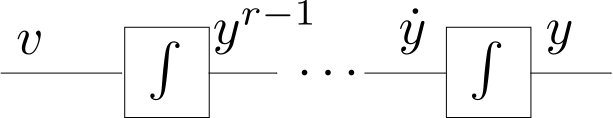
\includegraphics[width=7.5cm]{im312.pdf}
\end{figure}
\item Stabilisierung, Rückführung \begin{align*} v = - \sum\limits_{i=0}^{r-1} a_i y^{(i)} \tag{5.4} \end{align*} führt auf lineare Differentialgleichung. \begin{align*} y^{(r)} + a_ry^{(r-1)} + \dots + a_1\dot y + a_0 y = 0. \end{align*}
Rückführung in Originalkoord.: \begin{align*} y^{(k)} = L_f^{k}h(x) \text{ für } k=0,\dots, r-1 \\ 
u = -\frac{1}{L_g L_f^{r-1} h(x)} \sum\limits_{k=0}^{r} a_k L_f^{k} h(x) \text{ mit } a_r:=1. \tag{5.5}
\end{align*}
Unklar: Was passiert mit $u-r$ Koord.?
\end{enumerate} 
\subsection{Byrnes-Isidori Normalform}
System $(5.1)$ habe im Punkt $p\in M$ den wohldefinierten relativen Grad $r\le n.$
\subsection*{Lemma 5.1:} In eine Umgebung von $p$  \begin{align*} \langle dL_f^i h, ad_{-f}^{j}g \rangle = \left\{\substack{0 \qquad \text{ für }\qquad i + j < r-1\\ L_gL_f^{r-1}h(x), \quad i+j = r-1}\right. \tag{5.6}\end{align*}
\subsection*{Begründung}
\begin{align*} r=1: & \quad i +j \le r-1 = 0 \rightarrow i= j = 0\\ 
& \langle dL_f^\circ h, ad_{-f}^\circ h \rangle = \langle dh,g\rangle = L_gh \\ 
r=2:& \quad i+j = 1 \\ 
& i=1, j=0: \langle dL_f^1 h, ad_{-f}^\circ g\rangle = \langle dL_fh,g\rangle = L_g L_f h\\ 
& i=0, j=1: \langle dL_f^\circ h,ad_{-f}^1 g\rangle = \langle dh, [-f,g] \rangle = \langle dh, -[f,g] \rangle \\ 
&\qquad \qquad = -\langle dh, [f,g]\rangle = -L_{[f,g]}h = -\underbrace{(L_f L_g h - L_g L_f h)}_{\equiv 0\text{ weil } i>1} = L_g L_f h
\end{align*}
\subsection*{Lemma 5.2:} Die Kovektoren $dh(p), dL_fh(p),\dots, dL_f^{r-1} h(p)$ und linear unabhängig. 
\subsection*{Beweis:} Wegen Lemma $5.1$ gilt \begin{align}
\underbrace{\begin{pmatrix} dh(p)\\ dL_fh(p)\\ \vdots\\ dL_f^{r-1}h(p)\end{pmatrix}}_{\in \mathbb{R}^{r\times n}} \cdot \underbrace{\left( g(p) ,ad_{-f}g(p),\dots, ad_{-f}^{r-1}g(p) \right)}_{\in \mathbb{R}^{r\times n}} = 
\underbrace{\begin{pmatrix}
0      &    0   & & \dots & L_g L_f^{r-1} h(p)\\ 
\vdots & \vdots & & \star \\ 
0      &    0   & & \\ 
0      & L_gL_f^{r-1}h(p) & \vdots\\ 
\underbrace{L_g}_{\ne 0}L_f^{r-1}&h(p)&\star&\dots&\star
\end{pmatrix}}_{\in \mathbb{R}^{r\times r}}
\end{align} Rang $= r$ weil $ L_g L_f^{r-1} h(p) \ne 0 $\\ 
$\Rightarrow \text{ Kovektor } dh(p) ,\dots, dL_f^{r-1} h(p) $ sind linear unabh. \\ 
$\Rightarrow \text{ Vektoren } g(p),\dots, ad_{-f}^{r-1} h(p) $ sind linear unabh.
\begin{align*}
\begin{pmatrix} c^T\\ c^T A\\ \vdots\\ 
\end{pmatrix}\cdot 
\left( b,Ab,\dots,A^{r-1}b  \right) = \begin{pmatrix} 
0     & \dots& 0 & c^T A^{r-1} b\\ 
\vdots&      &   &  \\ 
0     &&&\vdots\\ 
c^TA^{r-1}b&\dots& &\star
\end{pmatrix}
\end{align*}
\subsection*{Lemma 5.3:} Wir setzen \begin{align*} 
\phi_1(x)&:= h(x)\\
\phi_2(x)&:= L_fh(x)\\ 
& \vdots\\ 
\phi_r(x)&:= L_f^{r-1}h(x) \end{align*} für $r<n$ gibt es $n-r$ weitere Funktionen $\phi_{r+1},\dots, \phi_{n},$ so dass 
\begin{align*}
\phi(x) = \begin{pmatrix} \phi_1(x)\\ \vdots\\ \phi_n(x) \end{pmatrix} \tag{5.7} 
\end{align*} im Punkt $p$ eine reguläre Jacobimatrix besetzt. Die zusätzliche Funktionen $\phi_{r+1},\dots, \phi_n$ können so gewählt werden, dass \begin{align*} L_g \phi_i(x) = d\phi_i(x) \cdot g(x) = 0, \qquad i=r+1,\dots, n \tag{5.8} \end{align*}
für alle $x$ aus einer Umgebung von $p$. \\ 
\subsection*{Hinweis:} (5.8) ist eine partielle Dgl.!
\subsection*{Beweis:} Es gilt $g(p) \ne 0, $weil rel. Grad wohldefininiert ist.
Damit ist die Distribution $\Delta = \text{span} [g]$ regulär , und weil $1.-$dim. auch involutiv: $[g,g] = g'g = g'g \equiv 0.$
\subsection*{Satz von Frobenius:} Es existieren $n-1$ SF  $\lambda_1, \dots, \lambda_{n-1}$ mit \begin{align*}\text{span} [d\lambda_1,\dots, d\lambda_{n-1}] = \Delta^\perp . \tag{5.9}\end{align*}
Wir wollen zeigen:
$\text{dim} (\underbrace{\Delta^{\perp}}_{dim \Delta^\perp = n-1} + \text{span}[\underbrace{dh}_{dim(\cdot) = r},\dots,dL_f^{r-1}h ]) = n$
im Punkt $p$.\\
Gleichbedeutend \begin{align*}\Delta^{\perp} + \text{span } [dh,\dots, dL_f^{r-1} h] = (\mathbb{R}^n)^\star \tag{*}\end{align*}
Orthogonales Komplement
\begin{align*}\underbrace{\Delta}_{\text{ span } [g]} \cap \text{ span} [dh, \dots, dL_f^{r-1} h]^{\perp} = [0] \tag{**} \end{align*}
Angenommen, $(**)$ gilt nicht, d.h. \begin{align*}
\underbrace{\Delta(p)}_{\text{span}[g(p)]} \cap \underbrace{\text{span}[dh, \dots, dL_f h^{r-1} ]^{\perp}}_{\text{ Annihilator}} \ne [0] \end{align*}
Dann muss $g(p)$ zum Annihilator gehören. Das ist nicht der Fall. \begin{align*}
\langle dL_f^{r-1} h(p) , g(p) \rangle = L_g L_f^{r-1} h(p)\ne 0
\end{align*}
Widerspruch: Damit gilt $(**)$ und damit $(*)$\\ 
Wegen Lemma 5.1 \begin{align*}
\text{dim span }[dh, \dots, dL_f^{r-1} h] = r,
\end{align*}anderseits wegen $(*)$: \\ 
\begin{align*} \text{dim span } [dh, \dots, dL_f^{r-1} ,d\lambda_1,\dots, d\lambda_{n-1}] = 0\end{align*}
Von den SF $\lambda_1,\dots, \lambda_{n-1} $ kann man $n-r$ zu Ergänzung der Basis wählen, O.E. $\lambda_1,\dots,\lambda_{n-r}:$
\begin{align*}
\text{dim span}[\underbrace{ dh, \dots, dL_f^{r-1}h }_{r}, \underbrace{d\lambda_1,\dots,d\lambda_{n-r}}_{n-r}] = n
\end{align*}
Folglich ist Jacobimatrix \begin{align*}
\phi'(p) = \begin{pmatrix} dh(p)\\ dL_f^{r-1} h(p)\\ d\lambda_1(p)\\ d\lambda_{n-r}(p) \end{pmatrix} \end{align*} regulär. Wegen $(5.9)$ folgt $(5.8)$
\subsection*{Satz 5.1:} Die in Lemma $5.3$ definierte Abbildung $\phi$ ist ein lokaler Diffeomorphismus, mit dem System 
\begin{align*}
\dot x &= f(x) + g(x) u\\ 
y &= h(x) \tag{5.1}
\end{align*}
in die Byrnes-Isidori-Normalform überführt wird:
\begin{align*}
\dot z_1 &= z_2\\ 
\vdots &\\ 
\dot z_{r-1} &= z_r\\ 
\dot z_r &= \alpha(z) + \beta(z)u\\ 
\vdots\\
\dot z_{r+1} &= q_1(z)\\
\dot z_n &= q_{n-r}(z)\\ 
y  &= z_1 \tag{5.10}
\end{align*}
\subsection*{Beweis: } Bei wohldefinierten relativen Grad $r$ ist $\phi'(p)$ regulär (Lemma 5.3)\\ 
$\Rightarrow  z= \phi(x) $ ist lokaler Diffeomorphismus 
\begin{itemize}
\item a) 1.TS: $z_i = \phi_i(x) = L_f^{i-1} h(x), \quad i=1,\dots, r$\\ Für $i=1,\dots, r-1$ gilt: \begin{align*}
\dot z_i = \frac{d}{dt} \phi_i(x) &= \phi_i'(x)\cdot \dot x\\ &=dL_f^{i-1}h(x)\cdot (f(x) + g(x) u)\\ 
&= L_f^i h(x) + \underbrace{L_g L_f^{i-1} h(x)}_{\equiv 0 \text{ weil } i< r } u\\ 
&= \phi_{i+1}(x) = z_{i+1} 
\end{align*}
Für $i = r $ gilt: \begin{align*} \dot z_r = \frac{d}{dt} \phi_r(x) &= \phi_r'(x)\cdot \dot x\\ 
&= dL_f^{r-1}h(x) \cdot (f(x) + g(x) u)\\ 
&= L_f^r h(x) + \underbrace{ L_g L_f^{r-1} h(x)}_{\ne 0} u 
\end{align*} 
T.S in $(5.10)$: \begin{align*} \alpha(z) &= L_f^r h(x)|_{x = \phi^{-1} (z)}\\ 
\beta(z) &= L_g L_f^{r-1} h(x)|_{x = \phi^{-1}(z)}
\end{align*}
\item b) 2.TS : $ z_i = \phi_i(x), \quad i = r+1,\dots, n. $ \begin{align*}
\dot z_i = \frac{d}{dt} \phi_i(x) = d\phi_i(x)\dot x &= d\phi_i(x)\cdot (f(x) + g(x) u)\\ &= L_f\phi_i(x) + \underbrace{L_g \phi_i(x)}_{\equiv 0 \text{ wegen (5.8)}}\cdot u = L_f \phi_i(x) =:q_{i-r}(z)|_{z = \phi(x)}
\end{align*}
$\Rightarrow q_i(z) = L_f \phi_{i+r}(x)|_{x = \phi^{-1} (z) } $. \\ 
Sei $z = \binom{\xi}{\eta} \begin{matrix}\leftarrow &r \\ \leftarrow &n-r \end{matrix} $Komponenten 
Normalform (5.10): \begin{align*}
\dot \xi &= A\xi + b\cdot (\alpha (\xi, \eta) + \beta (\xi, \eta) u)\\ 
\dot \eta &= q(\xi, \eta)\\
y&= c^T \xi \tag{5.11}
\end{align*}
\begin{align*}
A= \begin{pmatrix} 0&1 &&\\ & \ddots&\ddots&\\ &&&1\\ &&&0\end{pmatrix}, \quad b = \begin{pmatrix} 0\\ \vdots\\  0\\ 1\end{pmatrix}\\ 
c^T = (0,\dots, 1)
\end{align*}
\end{itemize} 
\subsection{Stabilisierung einer Ruhelage}
Im Punkt $p \in M $ gelte: \begin{align*} f(p) &= 0 \qquad \text{Ruhelage}\\ h(p)&= 0. \end{align*} 
Transformation $\phi$ kann so gewählt werden, dass $\phi(p) = 0.$Für $n=0$ ist dann $(\xi, \eta) = (0, 0)$ ebenfalls eine Ruhelage.
\begin{itemize}
\item a) Linearisierende Rückführung für 1.TS: \begin{align*}
u = \frac{1}{\beta(\xi, \eta)} (v - \alpha(\xi, \eta)) = \frac{1}{L_g L_f^{r-1} h(x)}(v - L_f^r h(x))
\end{align*} liefert für $(5.11):$
\begin{align*}
\dot \xi &= A\xi + b\cdot v\quad \text{ lineares System}\\ 
\dot \eta &= q(\xi, \eta) \quad \text{ interne Dynamik }\\ 
y &= c^T \xi \tag{5.12}
\end{align*}
\item b) Stabilisierung des 1.TS: Zustandsrückführung \begin{align*}
v&= k^T\xi , \quad k^T = (k_0,\dots, k_{r-1}) \\ 
\dot \xi &= (A - bk^T)\xi 
\end{align*}mit 
\begin{align*}
A - bk^T = \begin{pmatrix} 0 & 1 & 0 &\dots & 0\\ \vdots &&&&0\\ 0 &&0 & 1\\ -k_0 & -k_1 &\dots& -k_{r-2}&-k_{r-1}  \end{pmatrix}
\end{align*}
Frobenius-Regelmatrix mit 
charakteristischen Polynom 
\begin{align*}
\text{ det}(sI - (A - bk^T)) =  k_0 + k_1 s + \dots + k_{r-1}s^{r-1} + s^r \tag{5.13}
\end{align*}
Originalkoordinaten: \begin{align*} 
\xi_1 &= h(x), \xi_2 = L_fh(x),\dots, \xi_r = L_f^{r-1}h(x)\\ 
v&= -k^T \xi = - \sum\limits_{i=1}^{r} rk_{i+1} \xi_i = - \sum\limits_{i=0}^{r-1}k_i L_f^i h(x)
\end{align*}
Zustandrückführung \begin{align*}
u = \frac{1}{L_g L_f^{r-1} h(x)} (v- L_f^r h(x)) = -\frac{1}{L_g L_f^{r-1} h(x)} \sum\limits_{i=0}^r k_i L_f^i h(x) \quad \text{mit } k_r: =1\tag{5.14}
\end{align*}
\item c) Interne Dynamik 2.TS: \begin{align*}
\dot \xi &= (A - bk^T)\xi\\ 
\dot \eta &= q(\xi,\eta) \tag{5.15}
\end{align*}
hat bei $(\xi, \eta) = (0,0) $ ebenfalls eine Ruhelage. Stabilität des Gesamtsystems wird von 2.TS in (5.15) bestimmt. Autonomes System \begin{align*} \dot \eta  = q(0, \eta) \tag{5.16} \end{align*} 
Die Dynamik von $(5.16)$ heisst \textbf{Nulldynamik (zero dynamics)} \begin{align*}
\xi = 0 &\iff y= 0, \dot y= 0,\dots, y^{r-1} =0\\ &\iff y\equiv 0
\end{align*}  
Das System heisst \textbf{minimalphasig}, wenn die Ruhelage $\eta = 0$ von $(5.16)$ asymptotisch stabil ist.
\end{itemize}
\subsection*{Satz 5.2 (Stabiliseriung einer Ruhelage):}System (5.1) habe in einer Ruhelage $p\in M$ den rel. Grad $r$. Ausserdem sei das System minimalphasig und alle Wurzeln des char. Polynoms (5.13) liegen in der offenen linken Halbebene. Verwendet man die Zustandsrueckfuehrung (5.14), dann ist die Ruhelage $p$ asymptotisch stabil
\subsection{Stabilisierung in eine Ausgangstrajektorie}
Ausgangsreferenztrajektorie \begin{align*}
y_{\text{ref}} :[0, \infty ) \to \mathbb{R} \dots
\end{align*} $r$ -mal stetig diffbar.\\
\textbf{Bisher: } $y \to 0 $ mit $u  = \frac{1}{\beta (\xi, \eta)} (-\alpha(\xi,\eta) - k^T \xi)$\\ 
für $t \to \infty$\\ 
\textbf{Jetzt: } $y \to y_{\text{ref}} :$ Ansatz: $u =\frac{1}{\beta(\xi,\eta)} (-\alpha(\xi,\eta) + y_{\text{ref}}^{(r)}(t) + \sum\limits_{i=0}^{r-1} k_i (y_{\text{ref} }^{(i)} - \xi_{i+1}))$\\ 
1.TS \begin{align*}
\dot \xi_1 &= \xi_2\\ 
\dot \xi_{r-1}&= \xi_r\\ 
\dot \xi_r &=y_{\text{ref}}^{(i)}(t) + \sum\limits_{i=0}^{r-1}k_i(y_{\text{ref}}^{(i)}(t) - \xi_{i+1})\\ 
y &= \xi_1\tag{5.17}
\end{align*}
Fehler zwischen System. und Regerenzausgang \begin{align*} \xi(t) := y(t) - y_{\text{ref}}(t) \end{align*} Für die Normalform-Koord. gilt: \begin{align*}
\xi_{i} = y^{(i-1)}, \quad i= 1,\dots,r
\end{align*}
letzte Zeile des 1.TS: \begin{align*}
y^{(r)} = y_{\text{ref}}^{(r)} - \sum\limits_{i=0}^{r-1} k_i \xi^{(i)}
\end{align*}
$\iff$ lineare Dgl. \begin{align*}
k_0 \xi + k_1 \dot \xi + \dots + k_{r-1}\xi^{(r-1)} + \xi^{(r)} = 0.
\end{align*}
Rückführung (5.17) in $x-$Koord. \begin{align*}
u = \frac{1}{L_g L_f^{r-1} h(x)} \sum\limits_{i=0}^{r} r_i(y_{\text{ref}}^{(i)} (t) - L_f^{i-1} h(x)) \quad \text{ mit } r_r =1
\end{align*}
\section{ Eingangs-Ausgangs-Linearisierung für allg. nichtlineare Systeme}
\subsection{ Relativer Grad und Eingangs-Ausgangs-Normalform}
System \begin{align*}
\dot x &= F(x,u) \\ 
y &= h(x) \tag{5.20}
\end{align*} 
eingangsabhängiges \begin{align*}
\text{VF } F: M\times \mathbb{R}\to \mathbb{R}^{n} \\ 
\text{SF } h: M\to \mathbb{R}, \text{ glatt}\\ 
M\le \mathbb{R}^n, \quad \text{offen }
\end{align*}
\subsection*{Definition 5.2: } System (5.20) hat im Punkt $p \in M$ den (verallg.) relativen Grad $r$, falls 
\begin{enumerate}
\item \begin{align*}
\frac{\partial L_F^k h(x,u)}{\partial u} = 0 \quad \text{ für } R = 0,\dots, r-1.
\end{align*}
alle $x$ aus Umgebung von $p$ und alle $u$, 
\item \begin{align*} \frac{\partial L_f^r h(p,u)}{\partial u} \ne 0 \end{align*}
\end{enumerate}
Interpretation:
\begin{align*}
y &= h(x)\\ 
\dot y&= \frac{\partial h(x)}{\partial x}\cdot \dot x\\ 
&= \frac{\partial h(x)}{\partial x} \cdot F(x,u)\\ 
&= L_F h (x,u)\\ 
& \frac{\partial L_F h(x,u)}{\partial u} \left\{ \begin{matrix} \ne 0& , r=1\\ \equiv 0& \text{ weiter diff.}\end{matrix} \right.
\end{align*}
\begin{align*}
\ddot y &= \frac{d}{dt} L_F h(x,u)\\ 
&= \frac{\partial L_F^h}{\partial x}\dot x +\underbrace{\frac{\partial L_F^h}{\partial u} }_{\equiv 0 \text{ für } r > 1} \dot u\\ 
&= dL_F h\cdot F(x,u) \\ 
&= L_F^2 h(x,u) \equiv L_F^2 h(x)\\ 
y^{r-1}&= L_F^{r-1}h(x,u) \equiv L_F^{r-1}h(x)\\ 
y^{(r)}&= L_F^rh(x,u) \quad \text{mit } \frac{\partial L_F^r h(x,u)}{\partial u} \ne 0
\end{align*}
\subsection*{Kurzfassung:}
\begin{align*}
r = \text{arg} \min\limits_{R}\{\frac{\partial }{\partial u} L_F^R h(x,u) \ne 0\}
\end{align*}
\subsection*{Lemma 5.4:} System (5.20) habe im Punkt $p \in M$ den (verallg.) rel. Grad $r$. Dann sind die Kovektoren \begin{align*}dh(p), dL_F h(p), \dots, dL_F^{r-1} h(p) \end{align*} linear abhängig.
\subsection*{Beweis: } Indirekt, Angenommen, $dL_F^{r-1} h(p) $ wäre von den Kovektoren $dh(p),\dots, dL_F^{r-2} h(p)$ linear abhängig, d.h. es gilt Konstanten $c_{R} \in \mathbb{R} $ mit \begin{align*}
dL_F^{r-1} h(p) \cdot F(p,u) = \sum\limits_{k=0}^{r-2} C_{k}\cdot dL_F^{k} h(p) \cdot F(p,u)
\end{align*}
\begin{align*}
\Rightarrow \underbrace{\frac{\partial }{\partial u} L_F^r h(p,u)  }_{\ne 0} = \sum\limits_{k=0}^{r-2}C_k \underbrace{\frac{\partial }{\partial u} L_F^{k+1} h(p)}_{\equiv 0} 
\end{align*}
also doch linear unabhängig. 
\subsection*{Satz 5.3: } System (5.20) habe im Punkt $p\in M$ den rel. Grad $r$. Dann existiert ein lokaler Diffeomorphismus $z = (\xi, \eta) = \phi(x), $ der (5.20) in die \textbf{Eingangs-Ausgangs-Normalform} überführt:
\begin{align*}
\dot \xi_1 &= \xi_2\\ 
\vdots\\ 
\dot \xi_{r-1}&= \xi_r\\ 
\dot \xi_r &= \alpha(\xi, \eta, u) \text{ mit } \frac{\partial \alpha}{\partial u}\ne 0\\
\dot \eta_1 &= q_1(\xi, \eta, u)\\ 
\vdots\\
\dot \eta_{n-r}&=q_{n-r} (\xi, \eta, u)\\ 
y &= \xi \tag{ 5.21} 
\end{align*}
\subsection*{Beweis: } $\phi_i (x) = L_F^{i-1} h(x) $ für $i = 1,\dots, r$ \\ 
$\Rightarrow  \quad d\phi_1, \dots, d\phi_r $ sind in $p \in M$ Lemma 5.4 linear unabhängig. \\ 
$\Rightarrow$ Es gilt $n-r$ weitere (glatte) Funktionen $\phi_{r+1} , \dots, \phi_r$,so dass 
$d\phi_1, \dots, d\phi_n$ in $p\in M$ linear unabhängig , d.h. Jacobimatrix $\phi'$ von 
\begin{align*}
\phi = \begin{pmatrix}
\phi_1\\ \vdots\\ \phi_n
\end{pmatrix} 
\end{align*}ist in $p\in M $ regulär
$\Rightarrow \quad \phi $ ist lokaler Diffeomorphismus \\ 
Neue Koord: \begin{align*} \xi_1 &= \phi_1(x), \quad \eta_1 = \phi_{r+1}(x)\\
\vdots\\ 
\xi_{r} &= \phi_{r}(x),\quad \eta_{n-1} = \phi_n(x)
\end{align*}
d.h. $(\xi,\eta) = \phi(x) .$
\subsection*{1.TS: } \begin{align*}
\dot \xi_i &= \frac{d}{dt}\xi_i \qquad i =1,\dots, r\\ 
&= \frac{d}{dt} \phi_i(x)\\ 
&= \frac{d}{dt} L_F^{i-1}h(x)\\ 
&= dL_F^{i-1}h(x) F(x,u)\\ 
&= L_F^i h(x,u)\\ 
&= \left\{ \begin{matrix}\xi_{i+1} & \text{ für } i=1,\dots, r-1\\ 
\alpha(\xi, \eta, u) & \text{ für } i= r
 \end{matrix} \right.
\end{align*}
mit $\alpha(\xi, \eta, u) = L_F^r h(\phi^{-1}(\xi, \eta), u)$.
\subsection*{2.TS: } \begin{align*}
\dot \eta_j &= \frac{d}{dt}\eta_j ,\quad j=1,\dots, n-r\\ 
&= \frac{d}{dt}\phi_{r+j}(x)\\ 
&= d\phi_{r+j}(x)\cdot \dot x\\ 
&= d\phi_{r+j}\cdot F(x,u)\\ 
&= L_F \phi_{r+j}(x,u)
\end{align*}
$\Rightarrow$ \begin{align*} q_j(\xi, \eta, u) = L_F\phi_{r+j} (\phi^{-1}(\xi, \eta,),u). \end{align*}
\subsection*{Folgerung: } $\alpha$ sei stetig diffbar. und $\xi_0 \in \mathbb{R}^r, \eta_0\in\mathbb{R}^{n-r}, u_0 \in \mathbb{R}$ und \begin{align*}
v_0 := \alpha(\xi_0, \eta_0 , u_0). \\ 
\end{align*}
wegen \begin{align*} \frac{\partial \alpha}{\partial u}\ne 0\end{align*}
existiert eine stetig diffbare Abbuldung $\alpha^{-1}$ mit \begin{align*}
\alpha(\xi, \eta, \alpha^{-1}(\xi, \eta, v)) = v
\end{align*}
für alle $\xi, \eta v $ aus eine Umgebung von $\xi_0, \eta_0, v_0.$
\begin{align*}
v \overset{!}{=}\alpha(\xi, \eta, u) \iff u = \alpha^{-1}(\xi, \eta, v)
\end{align*}
Resultierendes 1.TS: \begin{align*}
\dot \xi_1 &= \xi_2\\ 
\vdots\\ 
\dot\xi_{r-1}&= \xi_r\\ 
\dot \xi_r &= v\\ 
y&= \xi_1\\
\iff \dot \xi &= A\xi + \underbrace{b}_{=e_n} v\\ 
y&= \underbrace{c^T}_{= e_1^T} \xi
\end{align*}
Zustandsrückführung zur Stabilisierung wie bei Byrnes-Isidori NF: 
\begin{align*}
v &= - K^T\xi, \text{ mit } k = (k_0, \dots, k_{r-1})^T\\ 
&= -\sum\limits_{i=0}^{r-1} k_i L_F^i h(x)
\end{align*}
\subsection*{Beispiel Schwebende Kugel im Magnetfeld:}
Eingang: Strom $I$\\ 
Ausgang: Position $y= l - l_0$\\ 
Bewegungsgl: $\ddot l\, m = mG - F$\\ 
Ansatz Kraft: $F = h \frac{I^2}{l^2}$
Zustandsraummodell mit $x = \binom{x_1}{x_2} = \binom{l}{\dot l}$
\begin{align*}
\binom{\dot x_1}{\dot x_2} = \begin{pmatrix}
x_2\\ 
G - \frac{\rho }{m} \cdot \frac{I^2}{x_1^2}
\end{pmatrix} =: F(x, I)
\end{align*}
\begin{align*}
y&= h(x)= l- l_0 = L_F^0 h(x)\\ 
\dot y&= \dot l = \dot x_1 = x_2 = L_F^1 h(x)\\ 
\ddot y&= \dot x_2 = G - \frac{\rho}{m}\cdot \frac{I^2}{x_1^2} = L_F^2 h(x, I) \qquad \textbf{ $ r=2$}\\ 
& \overset{!}{=} v
\end{align*}
Linearisierende Rückführung:
\begin{align*}
I^2 &= \frac{m}{\rho} x_1^2 (G - v)\\ 
I&= \underbrace{\pm}_{\substack{\text{Vorzeichen}\\ \text{Strom egal}}} \underbrace{\sqrt{\frac{m}{\rho} x_1^2 (G- v)}}_{ \text{ im für } \ge 0 \text{ def.} }
\end{align*}
Stabilisierung 
\begin{align*}
v = -k_0 x_1 - k_1 x_2 ; \qquad \underset{\text{Stotodola-Bed.}}{k_0, k_1 > 0}
\end{align*}
Charakt. Polynom
\begin{align*}
s^2 + k_1s + k_0
\end{align*}
\begin{align*}
I &= \sqrt{\frac{m}{\rho} x_1^2 (G + a_0 y + a_1 \dot y)}\\ 
&=\sqrt{\frac{m}{\rho} l^2 (G + a_0 (l- l_0) + a_1 \dot l)}
\end{align*}
mit modifizierter Wurzelfkt.
image1712
\subsection{Byrnes-Isidori-NF für nicht eingangsaffine Systeme}
Frage: Kann die Transformation $z = (\xi, \eta) = \phi(x)$ von (5.20) in die E/A -NF (5.21) so gewählt werden, daß das 2.TS nicht explizit vom Eingang $u$ abhängt?
\subsection*{Byrnes-Isidori-NF}
nichtaffine Systeme: \begin{align*}
\dot x_1 &= \xi_2\\ 
\vdots\\ 
\dot \xi_{r-1}&= \xi_r\\ \tag{5.22}
\dot \xi_r &= \alpha(\xi, \eta, u)\\ 
\dot \eta_1 &= q_1(\xi,\eta)\\ 
\vdots\\ 
\dot \eta_{n-r} &= q_{n-r}(\xi, \eta)\\ 
y &= \xi_1
\end{align*}
Alternative Darstellung von (5.22)\begin{align*}
\dot z &= z_2\frac{\partial}{\partial z_1} + z_r \frac{\partial }{\partial z_{r-1}} + \alpha(z,u)\frac{\partial}{\partial z_r}\\ 
&+q_1(z)\frac{\partial}{\partial z_{r+1}} + \dots + q_{n-r}\frac{\partial}{\partial z_n} \tag{5.23}
\end{align*}
\subsection*{Nichtaffines System}
\footnote{07.01.2015} 
\begin{align*}
\dot x &= F(x,u)\\ 
y &= h(x) \tag{5.20}
\end{align*}
\subsection*{Byrnes-Isidori-NF} für nichtaffine Systeme: 
\begin{align*}
\dot \xi_1 &= \xi_2\\ 
\vdots\\ \tag{5.22}
\dot \xi_{r-1}& = \xi_r\\ 
\dot \xi_r &= \alpha(\xi, \eta, u) = \frac{\partial \alpha (\xi, \eta, u)}{\partial u} \ne 0 \\ 
\dot \eta_1 &= q_1(\xi, \eta)\\ 
y &= \xi_1
\end{align*}
Alternative Darstellung von $(5.22):$
\begin{align*}
\dot z = z_2\frac{\partial}{\partial z_1} + \dots + z_r\frac{\partial}{\partial z_{r-1}} + \alpha(z,u)\frac{\partial}{\partial z_r} + q_1(z)\frac{\partial}{\partial z_{r+1}} + \dots + q_{n-r}\frac{\partial}{\partial z_n} \tag{5.23}
\end{align*}
\begin{itemize}
\item $n-1$ eingangsunabhängige Vektorfeld VF
\item genau 1 eingangsabhängige Skalarfeld SF
\end{itemize}
SISO-System $(5.20)$ kann für große $m$ immer folgendermaßen dargestellt werden:
\begin{align*}
\dot x = F(x,u) = f(x) + \sum\limits_{i=1}^{m} g_i(x)\varrho_i(x,u)
\end{align*}
mit eingangsunabhängigen Skalarfeldern $\varrho_1,\dots, \varrho_m$ und linear unhängigen VF $g_1, \dots, g_m.$\\ 
Transformation $z = \phi(x) $ liefert \begin{align*}
\dot z_j &= \frac{d}{dt}\phi_j(x)\\ 
&=d\phi_j(x)\cdot \dot x\\ 
&= d\phi_j(x)\cdot(f(x) + \sum\limits_{i=1}^{m}g_i(x) \varrho(x,u)) \qquad \text{ für  } j= 1,\dots, n\end{align*}
Damit der Eingang nur bei einem SF auftritt  $(Nr, R)$, muss für alle $j \in \{ 1,\dots, n\}\backslash \{R\}$ gelten. 
\begin{align*}
d\phi_j(x) \cdot (g_1(x) ,\dots, g_m(x))\equiv (0,\dots, 0)
\end{align*}
\begin{itemize}
\item sind $m$ partielle Dgln. pro Komponente $\phi_j$ 
\item Satz von Frobenius: $\exists$ höchstens $n-m$ unabhängige Lösungen
\item Für Invertierbarkeit sind $n-1$ SF $\phi_j$ mit l.n. Gradienten notwendig $\Rightarrow$ Es muß $m=1$ gelten.
\end{itemize}
\subsection*{Satz 5.4:} System $(5.20)$ habe den rel. Grad $r$. Es ex. genau dann eine Zustandstransformation in die Byrnes-Isidori-NF $(5.20)$, wenn das System $(5.20)$ in die Form \begin{align*}
\dot x = f(x) + g(x)\varrho(x,u) \tag{5.24} \end{align*} mit einem eingangabh. SF $\varrho$ und $g(x)\ne 0 $ überführt werden kann.\\ 
Beweisskizze: $\Rightarrow $ analog BI-NF für affine System $(5.1)$, insb. ist span$\{g\}$ involutiv.\\ 
$\Leftarrow $ Es gäbe die BI-NF $(5.22)$. Rücktransformation von $(5.23)$ liefert $(5.24)$. 
\subsection*{Bsp. (Rakete): } Zustand $x = (r, \dot r , \theta, \dot \theta)^T,$\\Eingang $n = \nu$ Antriebswinkel
\begin{align*}
\dot x = \underbrace{\begin{pmatrix}
x_2\\ -gR^2/x_1^2 + x_1 x_4^2\\ x_4\\  -2 x_2 x_4/x_1
\end{pmatrix}}_{f(x)} + \underbrace{\begin{pmatrix} 0 \\ F/m \\ 0 \\ 0\end{pmatrix}}_{g_1(x)} \cos{u} + \underbrace{\begin{pmatrix} 0\\ 0\\ 0\\F m_1/x_1\end{pmatrix}}_{g_2(x)} \sin{u}
\end{align*}
dim span $\{ g_1, g_2 \} = 2$\\ 
$\Rightarrow $ System kann NICHT in BI-NF überführt werden.\\ 
\subsection*{Alternative Herangehensweise:}
Überführung des nichtaffinen Systems $\dot x = F(x,u)$ durch Erweitern des Zustandes in ein eingangsaffinen System. \begin{align*}
\dot x &= F(x,u)\\ 
\dot u &= w 
\end{align*}
image701\\ 
neuer Zustand $\tilde x := \binom{x}{u}$\\ 
neuer Eingang $\tilde u := w. $
\begin{align*}
\dot{\tilde x} = \binom{\dot x}{\dot u} = \binom{F(\overbrace{x,u}^{\tilde x})}{w} = \binom{F(\tilde x)}{0} + \binom{0}{1}\tilde w
\end{align*}
\section{Exakte Eingangs-Zustands-Linearisierung}
Bisher: System mit rel. Grad $r\le n \Rightarrow $
\begin{itemize}
\item $r$-dim. lineares Teilsystem
\item $(n-r)-$dim. (in der Regel) nichtlineares TS
\end{itemize}
\subsection*{Frage:} Wann kann ein System
\begin{align*}
\dot x = f(x) + g(x)u \tag{5.1}
\end{align*} vollständig in ein lineares System überführt werden?
\subsection*{Festellung:} Das Problem der sog. \textbf{Eingangs-Zustands-Linearisierung} ist lösbar, wenn es eine Ausgangsabh. $h$ (d.h. ein SF) gibt, für welches das System den rel. Grad $n$ besitzt.\\ 
Ein solches System heißt \textbf{eingangs.-zustands-linearisierbar}.\\ 
Nach Def. 5.1 muß für $r=n$ gelten: \begin{align*}
L_g L_f^i h(x) \equiv 0 \qquad \text{ für } 0\le i \le n-2 \\ 
L_g L_f^{n-1} h(p) \ne 0 \tag{5.25}
\end{align*}
\subsection*{Lemma 5.1:} Für rel. Grad $r$ \begin{align*}
\langle dL_f^j h, ad_{-f}^i g \rangle = \left\{ \begin{matrix} L_g L_f^{r-1} h \quad \text{ für } i+j = r-1\\ 0 \qquad \text{ für } i+j < r-1 \end{matrix} \right.
\end{align*}
Für $j=0$:
\begin{align*}
\underbrace{\langle dh, ad_{-f}^i g \rangle }_{\equiv L_{ad_{-f}^i g} h}= \left\{ \begin{matrix} L_g L_f^{r-1} h \quad \text{ für } i = r-1\\ 0 \qquad \text{ für } i< r-1 \end{matrix} \right.
\end{align*}
Gleichwertige Formalisierung von Gl. $(5.25):$
\begin{align*}
L_{ad_{-f}^i g} h(x) \equiv 0 \quad \text{ für } 0\le i\le n-2\\ 
L_{ad_{-f}^{n-1} g} h(p)\ne 0 \tag{5.26}
\end{align*}
Die ersten $n-1$ Gln. von $(5.26)$: \begin{align*}
dh(x)\cdot (g(x), ad_{-f}g(x), \dots, ad_{-f}^{n-2} g(x) )\equiv (0,0,\dots,0) \tag{5.27}
\end{align*}
partielle Dgl. 1.Ordnung in $h$.
\subsection*{Distribution:}
\begin{align*}
\Delta_i(x) = \text{span}\{ g(x) ,ad_{-f}g(x) ,\dots, ad_{-f}^{i-1}g(x)\}
\end{align*}
\subsection*{Satz 5.5:} Wir betrachten System $(5.1)$ in Punkt $p \in M.$ Es existiert genau ein Ausgang mit rel. Grad $n$, wenn 
\begin{enumerate}[a)]
\item $\Delta_{n-1} $ involutiv ist und 
\item dim$\Delta_n(p) = n$
\end{enumerate}
\subsection*{Beweis:} $\Leftarrow$ Bedingungen $a) $ und $b) $ seinen erfüllt. \\ 
Wegen (b) ist auch $\Delta_{n-1}$ regulär mit dim$ \Delta_{n-1} = n-1, $\\ 
Wegen (a) auch involutiv Satz von Frobenius: \\ 
Es ex. ein SF $h$, welches alle VF von $\Delta_{n-1} $ annihiliert, d.h. \begin{align*}
0 \equiv \langle dh, ad_{-f}^i g \rangle = L_{ad_{-f}^i g} h. \text{ für } i = 0,\dots, n-2 \tag{*}
\end{align*}
Außerdem gilt \begin{align*}
0 \ne \langle dh, ad_{-f}^{n-1} \rangle (p) = L_{ad_{-f}^{n-1} g}h(p),  \tag{**}
\end{align*}denn sonst würde $dh$ Annihilator von $n$ linear unabh. VF seinen zu Dimensionsformel \begin{align*}(\text{dim} \Delta + \text{dim} \Delta^{\perp} = n)\end{align*}
Lineares System: 
\begin{align*}
\dot x &= \underbrace{Ax}_{f(x)} + \underbrace{h}_{g(x) \dots \text{konst}} u
\end{align*}
\begin{align*}
ad_{-f}g = [-f,g] &= -[f,g]\\ 
&= -(\underbrace{g'}_{\equiv 0}f - f'g)\\ 
&= f'\cdot g = Ab
\end{align*}
\begin{align*}
ad_{-f}^k g = A^k b
\end{align*}
\begin{align*}
\Rightarrow \Delta_n &= \text{span }\{ b, Ab, \dots, A^{n-1}b\}\\ 
\Rightarrow \Delta_n &=\text{im} Q_s
\end{align*}Steuerbarkeitsmatrix (Kalman) \begin{align*}
Q_s = (b, Ab, \dots, A^{n-1}b)
\end{align*}Für ein lin. System existiert genau dann ein Ausgang mit rel. Grad $n$ das System steuerbar ist.\\ 
Bedingung b) bedeutet, dass die \textbf{Steuerbarkeits} bzw. \textbf{Erreichbarkeitsmatrix} \begin{align*}
Q_s(x) = (g(x), ad_{-f}g(x), \dots, ad_{-f}^{n-1} g(x) )
\end{align*}regulär ist. 
\subsection*{Folgerung:}Für ein System mit $n=2$ ex. genau dann ein Ausgang mit rel. Grad $r=n$, wenn \begin{align*}
Q_s = (g(x), ad_{-f}g(x))
\end{align*} regulär ist.
\subsection*{Begründung:} 
\begin{itemize}
\item dim$ \Delta_n = \text{im } Q_s = n \qquad \text{weil regulär}$
\item $\Delta_{n-1} = \text{span} \{ g\} $ ist als 1.-dim Distribution involutiv $([g,g]\equiv 0)$
\end{itemize}
\begin{align*}
\dot z_1 &= z_2\\ 
\vdots\\ 
\dot z_{n-1} &= z_n\\ 
\dot z_{n} &= \alpha(z) + \beta(z)u\\ 
y &= z_1 \tag{5.28}
\end{align*}
\begin{align*}
\alpha(z) &= L_f^n h(x)\\ 
\beta(z) &= L_g L_f^{n-1}h(x) \ne 0.
\end{align*}
Für rel. Grad $r=n$ geht die Byrnes-Isidori-NF (5.10) in die \textbf{nichtlineare Regelungsnormalform (controller canonical form)} über:
\subsection*{Satz 5.6:} Für ein allg. nichtlineare System \begin{align*} \dot x = F(x, u) \tag{5.29} \end{align*} mit VF $F: M\times \mathbb{R} \to \mathbb{R}^n,$ glatt, $M \le \mathbb{R}^n $ offen sind folgende Aussagenäquivalent.
\begin{enumerate}[(a)]
\item System (5.29) ist eingangszustandslinearisierbar,
\item Es existiert ein eingangsabh. SF $\varrho$, so daß (5.29) in die Form \begin{align*} \dot x = f(x) + g(x)\varrho(x,u) \end{align*}
überführt werden kann, so daß System $(f,g)$ eingangs-zustands linearisierbar ist.


\item Das erweiterte Sytem \begin{align*}
\dot x &= F(u,w)\\ 
\dot u &= w
\dot{\tilde x} = \underbrace{\binom{F(x,u)}{0}}_{f(\tilde x)} + \underbrace{\binom{0}{1}}_{g(\tilde x)}
\end{align*}ist eingangs-zustand


\end{enumerate}
\section{Relativer Grad und Flachheit im Eingrößenfall}
\subsection*{Def.:}Das Eingrößensystem \begin{align*}
\dot x = F(x,u)
\end{align*}heißt \textbf{(differentiell) flach}, falls ein SF $\lambda: M\le \mathbb{R}^n \to \mathbb{R}$ existiert, so daß für \begin{align*}
z_1 = \lambda(x) \qquad \text{ flacher Ausgang}
\end{align*}
glatte Funktion $\psi, \theta$ existiert, so daß \begin{align*}
x &= \psi(z_1, \dot z_1, \dots, z_1^{(n-1)})\\ 
u &= \theta(z_1, \dot z_1, \dots, z_1^{(n)}).
\end{align*}
\subsection*{Satz 5.7:}Ein System \begin{align*}
\dot x = f(x) + g(x)u \tag{5.1}
\end{align*}ist genau dann flach, wenn es exakt eingangs-zustands-linearisierbar ist, d.h. wenn es ein SF \begin{align*}\lambda: M\to \mathbb{R} \end{align*}gibt, so daß das System den rel. Grad $n$ besitzt.\\ 
Koordin. -Transformation kann direkt angegeben werden. \begin{align*}
z = \begin{pmatrix} z_1\\ z_2 \\ \vdots\\ z_n \end{pmatrix} = \begin{pmatrix} z_1\\ \dot z_1\\ \vdots\\ z_1^{(n-1)}\end{pmatrix} = \begin{pmatrix}\lambda(x)\\ L_f \lambda(x)\\ \vdots\\ L_f^{n-1}\lambda(x)\end{pmatrix} = \phi(x)
\end{align*}Umkehrabb. \begin{align*} x = \psi(z)\end{align*}Jakobimatrizen \begin{align*}\frac{\partial z}{\partial x} = \phi'(x) \quad \text{bzw. } \frac{\partial x}{\partial z} = \psi'(z) \end{align*} sind regulär $(\Rightarrow \phi, \psi \text{ sind Diffeomorphisinen})$
\subsection*{Satz 5.8 (Hagenmager, Zeitz, 2004):}Wir betrachten System (5.1) mit $2$ Ausgängen: \begin{align*}
y&= h(x)\dots \text{ rel. Grad $r$ (Systemausgang)}\\ 
z_1&=\lambda(x)\dots \text{ rel. Grad $n$ (flacher Ausgang)}
\end{align*}Dann kann der Systemausgang wie 


\begin{align*}
y = \varrho(z_1, \dot z_1, \dots, z_1^{(n-r)}).
\end{align*}
\subsection*{Beweis:}Relativer Grad $n$ von $\lambda$ impliziert (Lemma 5.1/5.2): \begin{align*}
\langle dL_f^j \lambda, ad_{-f}^i g \rangle = \left\{\begin{matrix} 0 & \text{ für } i + j < n-1\\ L_gL_f^{n-1} \lambda & i+j=n-1\end{matrix}  \right.
\end{align*}
Also gilt: \begin{align*}
\underbrace{\begin{pmatrix}d\lambda\\ dL_f\lambda\\ \vdots\\ dL_f^{n-1}\lambda\end{pmatrix} }_{\frac{\partial z}{\partial x} = \phi'(x)}\cdot (g, ad_{-f} g, \dots, ad_{-f}^{n-1} g) = \underbrace{\begin{pmatrix} 0 & \dots & L_gL_f^{n-1}\lambda\\ \vdots & & \star\\ 0 && \\ L_gL_f^{n-1}\lambda & \star &\star \end{pmatrix}}_{\text{ regulär }} \tag{ *}
\end{align*}
Inverse einer rechten unteren $\Delta-$Matrix ist eine linke obere Dreieckmatrix \begin{align*}
\begin{pmatrix}
0 & \star\\ &\vdots\\ \star & \star \end{pmatrix}^{-1} = \begin{pmatrix} \star & \star\\ \star & 0\end{pmatrix} \tag{ **}
\end{align*}
Multiplikation von $(*)$ von links mit $\frac{\partial x}{\partial z}$ und von rechts mit der Inversen aus $(**)$: \begin{align*}
(g, ad_{-f}g, \dots, ad_{-f}^{n-1} g)\cdot \begin{pmatrix} \star & \dots & \star\\ \vdots & & \\ \star & &0\end{pmatrix} = \frac{\partial x}{\partial z} = \psi'(z) 
\end{align*}Für gilt wegen Lemma 5.1: \begin{align*}
\langle L_f^j h \text{verpasst}
\end{align*}
Damit \begin{align*}
dh\cdot (g, ad_{-f}g, \dots, ad_{-f}^{n-1} g) = (\underbrace{0,\dots, 0}_{r-1} ,\underbrace{\overbrace{*}^{\ne 0},\dots, 0}_{n-r+1})
\end{align*}
% Gradient der Ausgangsabb. in $z-$Koord.: \begin{align*}
% \frac{\partial h (\overbrace{\psi(z)}^{x})} &= h'(x)\cdot \psi'(z)\\ 
% &=h'(x)\cdot (g, ad_{-f}g,\dots, ad_{-f}^{n-1}g)\begin{pmatrix}\star &\dots&\star\\ \star &&\\ \star &&0\end{pmatrix} \\ 
% &=(\underbrace{0,\dots, 0}_{r-1}, \underbrace{*,\dots, *}_{n-r+1})\cdot \begin{pmatrix}\star &\dots&\star\\ \star &&\\ \star &&0\end{pmatrix}\\ 
% &=(\underbrace{*,\dots, *}_{n-r+1}, \underbrace{0,\dots, 0}_{r-1}_{r-1}),
% \end{align*}
d.h. die Asugangsabb. $h$ hängt nur von den ersten $n-r+1$ Komponenten
von $z$ ab, d.h. von \begin{align*}
z_1, z_2 = \dot z_1, \dots, z_{n-r+1} = z_1^{(n-r)}
\end{align*}
Ergänzung zur Eingangs-Zustands-Linearisierung: \begin{align*}
L_g h(x) = 0, L_{ad_{-f}g} h(x) = 0,\dots, L_{ad_{-f}^{n-2} g}h(x)= 0 \tag{I}
\end{align*}
und \begin{align*}
\underbrace{L_{ad_{-f}^{n-1}g}h(x)}_{= L_g L_f^{n-1} h(x) = \beta(z)\ne 0}\ne 0 \tag{II}
\end{align*}
Bisher: Nutzung von Bed. $(I)$, führt auf partielle Dgl. 
verpasst

Jetzt: Falls $\beta$ bekannt, Festlegung $1 \equiv \beta(z) = L_gL_f^{n-1} h(x)$ Bed $(I) + (II) $ ($n$ Dgl.): 
\begin{align*}
dh(x)\cdot (\underbrace{g(x), ad_{-f}g(x), \dots, ad_{-f}^{n-1} g(x)}_{=Q_s (x), n\times n})= e_n^T\\ 
\iff dh(x) =  e_n^T Q_s^{-1} 
\end{align*}$Q_s$ regulär\\ 
Vorgehen: 
\begin{itemize}
\item Berechnung der letzten Zeile der inversen Steuerbarkeitsmatrix \begin{align*} w(x) = e_n^T Q_s^{-1}(x)\end{align*} 
\item \begin{itemize}
\item $w$ geschlossen? 
\item verpasst
\end{itemize}
\end{itemize}
\chapter{Beobachterentwurf}
\section{Beobachtbarkeit}
System 
\begin{align*}
\dot x &= f(x)\qquad, x(0) = x_0 \in M\\ 
y &= h(x) \tag{6.1}
\end{align*}
$M \subset \mathbb{R}^n $ offen, \begin{align*}
VF: &f:M\to \mathbb{R}^n, \quad \varphi \dots \text{ Fluss}\\ 
SF: &h:M\to \mathbb{R}
\end{align*}
\subsection*{Def. 6.1:}Gegeben sei (6.1) und $T>0$. Zwei Anfangszustände $x_a, x_b \in \mathbb{R}, x_a\ne x_b$, heissen \textbf{nichtunterscheidbar}, wenn $\forall t\in [0, \tau]: h(\varphi_t(x_a)) = h(\varphi_t(x_b))$.\\
\footnote{21.01.2015}
Andernfalls heißen die Zustände \textbf{unterscheidbar}, d.h. wenn $\exists t\in [0, \tau]: h(\varphi_t(x_a))\ne h(\varphi_t(x_b)).$\\ 
image2101
\subsection*{Def.6.2:}System (6.1) heißt \textbf{(global) beobachtbar}, wenn es in $\mathbb{M}$ keine nichtunterscheidbaren Zustände gibt. 
\subsection*{Def.6.3:}System (6.1) heißt \textbf{lokal beobachtbar} im Punkt $x_0 \in \mathbb{R}$, wenn es eine Umgebung $U$ von $x_0$ gibt, die keine nichtunterscheidbaren Zustände enthält. System heißt \textbf{lokal boebachtbar,} wenn es für alle $x_0\in \mathbb{M}$ lokal beobachtbar ist. 
\subsection*{Motivation:} Zwei analyt. Kurven stimmen überein, wenn alle Taylorkoeff. gleiche Potenz übereinstimmen, statt Taylorkoeff: Ableitungen.\\ 
Lie- Reihe: \begin{align*}
y(t) = \sum\limits_{k=0}^{\infty} L_f^k h(x_0)\frac{t^k}{k!}
\end{align*}
\textbf{Beobachtbarkeitsabbildung} für $k \in \mathbb{N}:$ \begin{align*}
q(x) = \begin{pmatrix} y\\ \dot y\\ \ddot y\\ \vdots\\ y^{k-1}\end{pmatrix} + \begin{pmatrix} h(x)\\ L_fh(x)\\ L_f^2h(x)\\ \vdots\\ L_f^{k-1}h(x)\end{pmatrix} 
\end{align*}
$q(x_a) \ne q(x_b):$ $x_a$ und $x_b$ sind unterscheidbar.\\ 
Injektivität der Beobachtbarkeitsmatrix kann mit Satz über die Unkehrfunktion geprüft werden. Jakobimatrix \begin{align*}
Q(x) = q'(x) = \begin{pmatrix} dh(x)\\ dL_fh(x)\\ \vdots\\ dL_f^{k-1}h(x)\end{pmatrix}
\end{align*}heißt \textbf{Beobachtbarkeitsmatrix.}\\ 
Heinreichende Bedingung für lokale Beobachtbarkeit: 
\subsection*{Satz 6.1:} Die Beobachtbarkeitsmatrix $Q$ habe für ein $k \in \mathbb{N}$ an der Stelle $x_0$ den Rang $n$. Dann ist das System (6.1) im Punkt $x_0$ lokal beobachtbar.
\section{High-Gain-Beobachter für autonome Systeme}
Die Beobachtbarkeitsmatrix sei für $k=n$ regulär, Dann ist die Beobachtbarkeitsabbildung $q$ ein (lokale) Diffeomorphismus \begin{align*}
z=q(x) = \begin{pmatrix} h(x)\\ L_fh(x)\\ \vdots\\ L_f^{n-1}h(x)\end{pmatrix}
\end{align*}
der System (6.1) in die Form \begin{align*}
\dot z_1 &= z_2\\ \dot z_2 &= z_3\\ \vdots\\ \dot z_{n-1}&= z_n\\ \dot z_n &= \alpha(z) \quad \text{mit } \alpha(z) = L_f^n h(q^{-1}(z))\\y &= z_1 
\end{align*}
überführt \textbf{(Beobachtbarkeits-NF, observability canonical form)}. \\ 
Matrix-Darstellung: \begin{align*} \dot z &= Az + b\alpha(z)\\ y&= c^T \end{align*} mit \begin{align*} A = \begin{pmatrix} 0& 1 &&\\ &\ddots&&\\ &&\ddots&1\\ &&&0 \end{pmatrix}, b= \begin{pmatrix} 0\\ \vdots\\ 0\\1\end{pmatrix} =e_n, c^T = (1, 0,\dots, 0) = e_1^T.
\end{align*} 
Ansatz für Beobachter mit konstanter Beobachterverstärkung $k\in \mathbb{R}^n$: \begin{align*}
\dot{\hat z} &= A \hat z = b \alpha(\hat z) + k(y - \hat y)\\ 
\hat y &= c^T \hat z\end{align*} Beobachtungsfehler $\tilde z = z - \hat z$ genügt der Fehlergleichung \begin{align*}
\dot{\tilde z} & = \dot z - \dot{\hat z}\\ 
&= Az + b\alpha(z) - A \hat z - b\alpha(\hat z) - k(\overbrace{y}^{c^Tz} - \overbrace{\hat y}^{c^T\hat z})\\ 
&= (A -K c^T) \tilde z + b(\alpha(z) - \alpha(\hat z))
\end{align*}
Punkt $\tilde z = 0$ ist eine Ruhelage der Fehlergleichung.\\ 
Stabilität: $\alpha$ genüge einer Lipschitz-Bed. d.h. \begin{align*}
\exists \gamma > 0: | \alpha(z) - \alpha(\hat z) | \le \gamma \cdot|z - \hat z| = \gamma |\tilde z|.
\end{align*}
Dann existiert eine Beobachterverstärkung $K \in \mathbb{R}^n$, so daß die Ruhelage $\tilde z = 0$ der Fehlergleichung exponentiell stabil ist. \\ 
Lineare Teil: Mit \begin{align*}
K = \begin{matrix} p_{n-1} \\ \vdots\\ p_0\end{matrix}\in \mathbb{R}^n 
\end{align*}enthält man das char. Polynom.
\begin{align*}
\text{det} (sI - (A - Kc^T)) = s^n + p_{n-1}s^{n-1} + \dots + p_1s + p_0
\end{align*}Implementierung des Beobachters in Originalkoord.: \\ 
Kettenregel \begin{align*}
\dot{\hat z} &= \frac{d}{dt} \hat z(t) &= \frac{d}{dt} q(x(t))\\ \dot{\hat x} &= Q^{-1}(\hat x)\cdot \dot{\hat z} &=\underbrace{ q'(\hat x (t))}_{Q(\hat x(t))} \cdot \dot{\hat x}(t)
\end{align*}\begin{align*}
&= \underbrace{Q^{-1}(\hat x) \cdot (A\hat z + b\alpha(\hat z)}_{f(\hat x)} + k(y - \hat y))\\ 
&= f(\hat x) + \underbrace{Q^{-1}(\hat x) k }_{=: l(\hat x)} (y(t) - h(\hat x))
\end{align*}
$\dots$ vom Schätz-bzw. Beobachterzustand abh. Verstärkung $l : \mathrm{M} \to \mathbb{R}^n (VF)$
\subsection*{Bsp:} \begin{align*}
\dot x_1 &= -x_2 + x_1 (1- x_1^2)\\ 
\dot x_2 &= x_1 + x_2(1- x_2^2)
\end{align*}
\begin{align*}
\left.\begin{matrix}
y &=& x_1 = h(x) \Rightarrow dh(x) = (1\,x) \\ 
\dot y&=& \dot x_1\\ 
&=& -x_2 + x_1(1-x_1)^2\\ 
&=& L_f h(x) \Rightarrow \quad dL_fh(x) = (1-3x_1^2, -1)\end{matrix}\right\}Q(x) = \begin{pmatrix} dh(x)\\ dL_fh(x)\end{pmatrix} = \begin{pmatrix} 1 & 0\\ 1- 3x_1^2 & -1\end{pmatrix}
\end{align*}
Charakt. Polynom: $s^2 + p_1 s + p_0, \qquad p_0, p_1 > 0 $
\begin{align*}
l(\hat x) = Q^{-1}(\hat x) \underbrace{\begin{pmatrix} p_1\\p_0\end{pmatrix}}_{k\in\mathbb{R}^2} =\begin{pmatrix} p_1\\ p_1(1-3\hat x_1^2) - p_0 \end{pmatrix} 
\end{align*}
Beobachter: \begin{align*}
\dot{\hat x} = \underbrace{\begin{pmatrix} - \hat x_2 + \hat x_1(1- \hat x_1^2)\\ \hat x_1 + \hat x_2(1-\hat x_2^2)\end{pmatrix}  }_{f(\hat x)} + \begin{pmatrix} p_1\\ p_1(1-3\hat x_1^2) - p_0\end{pmatrix} \cdot (y(t) - \hat x_1) 
\end{align*}
\section{High-Gain-Beobachter für nichtautonome Systeme}System \begin{align*}
\dot x &= f(x) + g(x)u\\ 
y&= h(x) \tag{6.2}
\end{align*}
VF: $f,g: \mathrm{M} \to \mathbb{R}^n$\\ 
SF: $h\, :\mathrm{M} \to \mathbb{R}$\\ 
Beobachtbarkeit kann vom Eingangssingal abhängen.\\ 
\subsection*{Bsp:} \begin{align*}
\dot x_1 &= -x_1 + x_2 u\\ 
\dot x_2 &= x_2\\ 
y &= x_1
\end{align*}
\begin{itemize}
\item a). $n=0:$ Ausgangskurve $y(t) = e^{-t}, \qquad x_1(0) $ hängt nur von $x_1 $ ab.\\  $\Rightarrow $nicht beobachtbar!
\item b). $n\ne 0$: System beobachtbar:\begin{align*} x_1&= y\\ x_2&= y + \dot y\end{align*}
\end{itemize}
\subsection*{Satz 6.2:} Bed. für lokale Beobachtbarkeit bei bel. Eingangssignal: System ist in folgende Form überführbar.

\begin{align*}
\dot z_1 &= z_2 + \beta_1 (z_1) u\\ 
\dot z_2 &= z_3 + \beta_2(z_1, z_2) u\\ 
\vdots\\ 
\dot z_n &= \alpha(z) + \beta_n(z_1, \dots, z_n)u\\ 
y &= z_1 \tag{6.3}
\end{align*}
Funktionale Abhängigkeit \begin{align*} \beta_1(z_1)\\ \beta_2(z_1,z_2)\end{align*} Lineare Abhängigkeit \begin{align*}
d\beta_1 \in \text{span }\{ dz_1\}\\ 
d\beta_2 \in \text{span }\{dz_1, dz_2\}
\end{align*}
Transf. von (6.2) durch Beobachtbarkeitsabb. 
\begin{align*}
z  = q(x), \quad z_i = L_f^{i-1}h(x), \quad i= 1,\dots n
\end{align*}
\begin{align*}
\begin{matrix}
\dot z_1 &=& \frac{d}{dt}h(x) &=& dh\dot x &=& dh(f + g u)\\ 
&& && &=&\underbrace{L_f h}_{z_2} + \underbrace{L_g h}_{\beta_1} \cdot u\\
\dot z_1 &=&\frac{d}{dt}L_fh(x) &=&dL_fh\cdot \dot x &=& dL_fh\cdot (f + gu)\\ 
&& && &=&\underbrace{L_f h}_{z_2} + \underbrace{L_f^2h}_{z_3} + \underbrace{L_g L_f h}_{z } u 
\end{matrix}
\end{align*}
Bed. für Form 6.3 \begin{align*}
dL_g L_f^i h \in \text{span }\{ dh, dL_f h, \dots, dL_f^i h \} \quad i =0, n-2
\end{align*}
\section{Exakte Linearisierung des Beobachtungsfehlers}
System \begin{align*}
\dot x &= F(x,u)\\ y &= h(x) \tag{6.4}
\end{align*}
Angenommen, $\exists$ Koordinatentransformation \begin{align*}
z = T(x), \quad x = S(z),
\end{align*} die System (6.4) in die \textbf{Beobachter-Normalform} überführt \begin{align*}
\dot z &= Az + \alpha(y,u)\\ 
y &= c^T z \tag{6.5}
\end{align*}
\begin{itemize}
\item lineare Ausgang
\item lineare Dynamik
\item \textbf{nichtlineare Eingangs-Ausgangs-Aufschaltung} \begin{align*}
\alpha: \mathrm{R}\times \mathrm{R}\to \mathrm{R}^n
\end{align*}
\end{itemize}
Das Paar $(A, c^T)$ sei beobachtbar, Form: \begin{align*}
A = \begin{pmatrix}
0 && 0\\ 1 &&\\ 
&\ddots&\\ 0&1&0
\end{pmatrix}\qquad
c^T = (0, \dots, 0, 1)\quad \text{Duale \textbf{Brunovsky Form}}
\end{align*}
Ansatz für Beobachter: 
\begin{align*}
\dot{\hat z} &= A \hat z + \alpha(y,u) + k\overbrace{(y - \hat y)}^{\text{Ausgangsfehler}}\\ 
\hat y &= c^T \hat z\\ 
\hat x &= S(\hat z) \tag{6.6}
\end{align*}
$k \in \mathrm{R}^n$ Konstante Beobachterverstärkung\\ 
Beobachtungsfehler $\tilde z = z - \hat z$ genügt der Fehlerdgl.:
\begin{align*}
\dot{\tilde z} &= \dot z - \dot{\hat z}\\ 
&= Az + \alpha(y,u) - A\hat z - \alpha(y,u) - kc^T(z-\hat z)\\ 
&= (A - kc^T)\tilde z \qquad \dots \text{ ist \textbf{exakt} linear!}
\end{align*}
Systemmatrix \begin{align*}
A - kc^T = \underbrace{\begin{pmatrix}
0 & \dots & 0 & -p_0\\ 
1 & \ddots&\vdots& \vdots\\ 
0 & \ddots& 0&-p_{n-2}\\ 
0&&&\\ 
0&\dots&1&-p_{n-1}
\end{pmatrix}}_{\text{Frobenius Begleitmatrix}}
k = \begin{pmatrix}
p_0\\ \vdots\\ p_{n-1}
\end{pmatrix}
\end{align*}
Beobachter (6.6) $\dots$ \textbf{Normalform Beobachter}
Beobachter (6.6) in $x$-Koord.: \begin{align*}
\dot{\hat x} &= \frac{x}{dt}S(\hat z)|_{(6.6)} \\ 
&= S'(\hat z)[ A\hat z + \alpha(y,u) + k(y- \hat y) ]\\ 
&= S'(\hat z)[ A\hat z + \alpha(\hat y,u)] + S'(\hat z)[\alpha(y,u) - \alpha(\hat y,u) + k(y- \hat y)]\\ 
&= F(\hat x,u) + \underbrace{[T'(\hat x)]^{-1}\cdot[\alpha(y,u) - \alpha(h(\hat x),u) - k(y- h(\hat x))]}_{=: R_{\infty} (\hat x, y,u)}
\end{align*}
\begin{align*}
z &= T(x), \quad x = S(z)\\ 
z &= T(S(z))\qquad|\frac{d}{dt}\\
I &= T'(x)S'(z)\\ 
\Rightarrow &= (T')^{-1} = S' 
\end{align*}
Schwierigkeit des Verfahrens: \\ 
Existenz bzw. Berechnung der Normalform bzw. der Koord-Transf.\\ 
Aufspaltung der rechten Seite von (6.4): \begin{align*}
F(x,u) = f(x) + g(x,u) \tag{6.8}
\end{align*}
mit \begin{align*}
f(x)&:= F(x,0)\\ 
g(x,u)&:= F(x,u) - F(x,0)
\end{align*}
\subsection*{Satz 6.2:}Das System \begin{align*}
\dot x = f(x) + g(x)u, \quad y= h(x) \tag{6.9}
\end{align*}
ist genau dann in einer Umgebung eines Punktes $p \in \mathrm{M}\subset \mathrm{R}^n$ durch eine Koord.-Transf. $z = T(x)$ bzw. $x = S(z)$ in die Beobachter-Normalform (6.5) überführbar, wenn folgende Bedingungen erfüllt sind: \begin{align*}
B1: &\text{dim }(dh(p), dL_fh(p),\dots, dL_f^{n-1} h(p)) = n,\\ 
B2: &[ad_{-f}^i  v, ad_{-f}^j v]\equiv 0\text{ für } 0\le i,j \le n-1,\\ 
B3: &[g, ad_{-f}^i v] \equiv 0 \text{ für } 0\le i \le n-2,
\end{align*}
wobei das Vektorfeld $v$ die eindeutige definierte Lösung von 
\begin{align*}
L_v L_f^i h(x) = \left\{
\begin{matrix} 0 &\text{ für } & i=0,\dots, n-2\\ 
1 & \text{ für } & i=n-1\end{matrix}
\right.
\end{align*}
\subsection*{Beweis:} Wir zeigen: B1-B3 sind hinreichend\begin{align*}
L_vL_f^{'}h(x) = \langle dL_f^i h, v \rangle (x)
\end{align*}Gl. (6.9) zeilenweise
\begin{align*}\underbrace{\begin{pmatrix}
dh(x)\\ dL_fh(x)\\ 
\vdots\\ dL_f^{n-1}h(x)
\end{pmatrix}}_{Q(x)} v(x) = \underbrace{\begin{pmatrix} 0\\ 0\\ \vdots\\ 0\\ 1\end{pmatrix}}_{e_n}\tag{6.10}
\end{align*}
Wegen B1 sind die Zeilen der Beobachtbarkeitsmatrix $Q$ linear unabhängig \begin{itemize}
\item $Q$ ist in Umgebung von $p$ invertierbar (regulär)
\item \begin{align*}v(x) = Q^{-1}(x) e_n   \tag{6.11} \end{align*}
\end{itemize}
$v(x)\dots$ Startvektor, letzte Spalte der inversen Beobachtbarkeitsmatrix\\ 
Aus (6.9) folgt (Lemma 5.1 (5.2)): \begin{align*}
\begin{pmatrix}
dh(p)\\ dL_fh(p)\\ \vdots\\ dL_f^{n-1}h(p)
\end{pmatrix}\cdot (v(p), ad_{-f}v(p),\dots) = \begin{pmatrix}
0 & \dots & 0 & 1\\ 
\vdots & &&*\\ 
0 &&&\vdots\\ 
1& * &\dots& *
\end{pmatrix}\tag{6.12}
\end{align*} 
\begin{itemize}
\item $n$ Vektoren $v(p), ad_{-f}v(p), \dots, ad_{-f}^{n-1}v(p)$ sind linear
\item $n$ VF $v(x), ad_{-f}^{n-1}v(x)$ sind linear unabhängig   
\end{itemize}
Zusammen mit B2 \begin{itemize}
\item Satz über simultane Begradingung von VF: Es ex. (lokaler) Diffeomorphismus \begin{align*}
z = T(x), x = S(z) \tag{ 6.13}
\end{align*}mit \begin{align*}
T_{*}ad_{-f}^{i}v = \frac{\partial }{\partial z_{i+1}} = e_{i+1}
\end{align*}
bzw. \begin{align*}
ad_{-f}^i v = S_{*} \frac{\partial }{\partial  z_{i+1}} &= S'(z) \frac{\partial}{\partial z_{i+1}}\\ 
&= \frac{\partial S(z)}{\partial z_{i+1}}
\end{align*}
System in transformatieren Koordn. : \begin{align*}
\bar f(z) &= T_{*} f(x)|_{x = S(z)}\\ 
\bar g(z,u) &= T_{*} g(x,u)|_{x = S(z)}\\ 
\bar h(z) &= h(x)|_{x= S(z)} \tag{6.14}
\end{align*}
\end{itemize}
Ausgangsabb $\bar h:$ \begin{align*}
\bar h (z) = h(S(z))
\end{align*}Wegen (6.13) gilt \begin{align*}
\frac{\partial \bar h}{\partial z_{i+1}} &= \frac{\partial h}{\partial x} \frac{\partial x}{\partial z_{i+1}}\\ 
&= dh(x) \cdot \frac{\partial S(z)}{\partial z_{i+1}}\\ 
&= dh(x) \cdot ad_{-f}^i v(x)\\ 
&= \langle dh, ad_{-f}^i v \rangle (x)\\ 
&= \left\{ \begin{matrix} 0 & \text{ für } & i = 0,\dots, n-2\\ 
1 & \text{ für }& i = n-1\end{matrix}
 \right.
\end{align*}
\begin{itemize}
\item \begin{align*}
d\bar h(z) \equiv (0, \dots, 0, 1) = e_n^T = c^T
\end{align*}
\item \begin{align*}
\bar h(z) = z_1 = c^T z. 
\end{align*}
\end{itemize}
Vektorfeld $\bar f$: Für $i = 1, \dots, n-1$ gilt \begin{align*}
e_{i+1} = \frac{\partial }{\partial z_{i+1}} &= T_{*}ad_{-f}^i v \\ 
& = T_{*} [-f, ad_{-f}^{i-1} v]\\ 
&= [-T_{*} f, T_{*} ad_{-f}^{i-1} v]\\ 
&= [-f, \underbrace{\frac{\partial}{\partial z_{i}}}_{e_i}], \qquad \frac{\partial e_i}{\partial z} = 0\\ 
&= \bar f'\cdot \frac{\partial }{\partial z_i} = \frac{\partial \bar f}{\partial z_i} \tag{6.15}
\end{align*}
Jacobimatrix hat Form
\begin{align*}
\bar f'(x) = \begin{pmatrix}
0 & 0 & &0& *\\ 
1 & 0 && \vdots&\vdots\\ 
0 & 1 && 0 &\vdots\\ 
\vdots&\vdots& & 0&\\ 
0&0 && 1 &*
\end{pmatrix}
\tag{6.16}
\end{align*}
\begin{itemize}
\item Gl. (6.13) für $i = 0, \dots, n-1$ zusammengefaßt: \begin{align*}
S'(z) = \underbrace{(v, ad_{-f} v, \dots, ad_{-f}^{n-1} v) }_{TT(x)}(x)|_{x = S(z)}
\end{align*}
System partieller Differentialgl. 1.Ordnung\\ 
Eine Lösung $S$ von (PDE) ist die Koordinatentrafo. 
\end{itemize}
\subsection*{Bemerkung:}
\begin{itemize}
\item B1 ist Beobachtbarkeitsrangbedingung
\item B2 nennt man Involutivitäts oder Integrabilitätsbedinung, ist für reale Systeme nicht erfüllt
\end{itemize}
\subsection*{Beispiel: }Rössler-System
\begin{align*}
\dot x_1 &= -x_2 - x_3\\ 
\dot x_2 &= x_1 + ax_2\\ 
\dot x_3 &= c + x_3(x_1 - b)\\ 
y &= lnx_3, \quad x>0
\end{align*}Chaot. Verhalten für \begin{align*} a &= 0.55\\ b &= 4\\ c&= 2\end{align*}
Beobachtbarkeitsmatrix: \begin{align*}
Q(x) = \begin{pmatrix} dh(x)\\ dL_fh(x)\\ dL_F^2h(x)\end{pmatrix} = \begin{pmatrix}
0 & 0 & \frac{1}{x_3}\\ 
1 & 0 & -\frac{c}{x_3^2}\\ 
-\frac{c}{x_3} & -1& \frac{cx_1 x_3 - bc x_3 + 2c^2 - x_3^3}{x_3^3}
\end{pmatrix}
\end{align*}Startbektor: \begin{align*}
v = Q^{-1} e_3 = \begin{pmatrix} 0 \\ -1\\ 0\end{pmatrix}
\end{align*}Jakobimatrix der Transformation: \begin{align*}
S'(z) &= (v, ad_{-f}v, ad_{-f}^2 v) \\ 
\text{Konstante} &= \begin{pmatrix}
0 & 1 & a\\ 
-1& -a& 1-a^2\\ 
0 & 0 & x_3
\end{pmatrix} \quad \text{ lin. VF}
\end{align*}
Über die Flüße erhält man die Koordn. Trafo: 
\begin{align*}
x &=S(z) = \begin{pmatrix} z_2 + az_3\\ -z_1 - az_2 + (1-a^2)z_3\\ exp z_3\end{pmatrix} \\ 
z &= T(z) = \begin{pmatrix} -a x_1 - x_1 + lnx_2\\ x_1 - a ln x_3\\ ln x_3 \end{pmatrix}
\end{align*}

\end{document}
